%EKG-7 Projektbericht

%****************************************************************************************************************%
% Hier stehen einige Hinweise für die Form die ich aktualisiere wenn mir was Wichtiges auffällt
%
% - Unter jede Überschrift muss wenigstens eine Einleitung
% - zwischen Zahlen und Einheiten muss ein Leerzeichen. Bsp für Einheiten im Fließtext sind in analoge Filterschaltung
% - Nicht mehr als 3 Überschriftsebenen
% - laut Chowanetz soll die Konzeptfindung und die genaue Erklärung des Moduls in verschiedene Unterkapitel getrennt werden. Am Ende von Kapitel 5.1 Konzeptfindung soll quasi das Blockschaltbild stehen, die Erklärung folgt dann in den Kapiteln danach
%
%****************************************************************************************************************%


\documentclass[a4paper, 12pt]{article}

\usepackage[ngerman]{babel}
\usepackage[utf8]{inputenc}
\usepackage[T1]{fontenc}
\usepackage{hyperref}
\usepackage{fontspec} %muss mit XeLaTex oder LuaLatex kompiliert werden sonst gibts Errors
%\setmainfont{Calibri} %Dieser Font scheint auf Appleprodukten Probleme zu bereiten
\usepackage[a4paper, right=2cm, top=2cm, left=3cm, bottom=3cm]{geometry}
\usepackage{setspace} %mit dem package kann der Zeilenabstand beeinflusst werden
\setstretch{1.3}  %Zeilenabstand 1.3-fach
\usepackage[%per=slash,
            decimalsymbol=comma,
            loctolang={DE:ngerman,UK:english},
            ]{siunitx} %für die Darstellung von Einheiten im Fliesstext
\usepackage{graphicx,wrapfig,lipsum} %für die Einbindung von Grafiken
\usepackage{subcaption}
\bibliographystyle{unsrt} %muss erst mit Bibtex und dann mit XeLaTex kompiliert werden

%Set Path for Graphics
\graphicspath{{Bilder/}}

%Set Path for Chapters
\makeatletter
\def\input@path{{./}{./Chapter/}}
\makeatother

\setlength{\parindent}{0em} %Kein Einzug bei einem neuen Absatz

\begin{document}

%ekg_7_Titelseite

\title{Georg-Simon-Ohm Hochschule Nürnberg\\Fakultät Elektrotechnik Feinwerktechnik Informationstechnik}
\author{Niklas Gampl\\Hannes Holzmann\\Adrian Jäger\\Ivan Kozlov\\Erik Thüry}
\date{\today}
\maketitle

\noindent
\begin{center}
    \Large{Projektarbeit zum Thema:\\
    Entwicklung eines mobilen, µC-gesteuerten EKG}
\end{center}
\normalsize

\vfill

\noindent
Semester: Wintersemester 20/21

\noindent
Abgabedatum: 10.03.2021

\noindent
Betreuer: Prof. Dr. Chowanetz

\thispagestyle{empty} %keine Seitenzahl anzeigen

\newpage

\tableofcontents %das Inhaltsverzeichnis aktualisiert sich erst nach zweimaligem kompilieren
\thispagestyle{empty} %keine Seitenzahl anzeigen

\newpage

%ekg_7 Abkürzungsverzeichnis

\section{Abkürzungsverzeichnis}

EKG - Elektrokardiogramm \\ FFT - Fast-Fourier-Transformation \\ SMD - Surface-mounted device \\ Test

\newpage

%ekg_7_Einleitung und Motivation

\section{Einleitung und Motivation}

Seit der Entdeckung der Methode zur Ableitung der elektrischen Potenziale am menschlichen Herzen hat die Diagnostik durch das Elektrokardiogramm (EKG) eine essentielle Bedeutung in Kliniken, Arztpraxen und im Rettungsdienst eingenommen. Für den Anwender ist es eine einfache, schnelle und vor allem nicht invasive Methode sich ein Bild vom Zustand der Erregungsleitung am Herzen des Patienten zu machen. Schwerwiegende Erkrankungen wie Infarkte oder Kammerflimmern können sofort diagnostiziert werden, wodurch die Therapie zeitnah eingeleitet werden kann. Doch auch in der Diagnostik von leichteren oder chronisch verlaufenden Krankheiten ist das EKG ein wichtiges Werkzeug im Repertoire des Arztes, wenn der Patient die Möglichkeit des Arztbesuchs auch wahr nimmt. Die wenigsten Patienten lassen sich ohne Symptome oder Leidensdruck rein prophylaktisch von ihrem Arzt untersuchen. Dabei beginnen die meisten schweren Erkrankungen mit einem symptomlosen Stadium, in welchem eine einfache Behandlung, zum Beispiel mit Medikamenten und ohne bleibende Schäden möglich wäre. So ist es auch im Fall der Volkskrankheit des Vorhofflimmerns von der in Deutschland etwa 300.000 Menschen betroffen sind. 

Im gesunden Herzen arbeiten Vorhöfe und Kammern zeitlich genau abgestimmt zusammen. Die Hauptlast der Pumpleistung übernehmen die Kammern. Diese können ihr volles Potential jedoch nur ausschöpfen, wenn die Vorhöfe kurz vor der Kammerkontraktion kontrahieren. Dass bewirkt die vollständige Füllung der Kammer und eine optimale Ausnutzung der Schlagkraft. Außerdem fließt das Blut so möglichst laminar, also ohne Verwirbelungen. 

Beim Vorhofflimmern kommt es zu einer unvollständigen Kontraktion der Vorhöfe. Durch eine gestörte Erregungsleitung am Herzen arbeiten die Muskelzellen nicht mehr synchron. Die Vorhöfe flimmern (manchmal spricht man auch vom "Flattern") nur noch, anstatt koordiniert zu kontrahieren. Die Kammer kann nicht mehr effizient arbeiten und das Blut bildet Turbulenzen. Zum einen führt dies zu einer verminderten Leistungsfähigkeit des Patienten, was in einem Teil der Fälle jedoch nicht bemerkt wird, zum anderen können durch die Verwirbelungen im Blut kleine Thromben entstehen. Diese Thromben, also Blutgerinnsel, werden aus der Kammer in den Blutkreislauf ausgeworfen und können sich je nach Herzseite im Kapillargebiet der Lunge oder des Gehirns festsetzen. So verstopfen sie die Blutzufuhr und das dahinter liegende Gewebe stirbt ab. Geschieht dies im Gehirn spricht man von einem Schlaganfall (Apoplex), der meist irreparable Schäden nach sich zieht. 

In unserem Projekt soll ein EKG-Gerät entwickelt werden, dass die Diagnose solcher stiller Herzerkrankungen ermöglicht, ohne dass der Patient dafür die Praxis des Arztes besuchen muss. So kann ein Mediziner im Nachhinein Aufnahmen von verschiedenen Tagen auswerten und mit einander vergleichen. Bei sporadisch auftretenden Symptomen ist die Möglichkeit jederzeit unabhängig ein EKG aufzeichnen zu können, besonders hilfreich für die Diagnose. Langfristig könnte die bessere Verfügbarkeit dieser Untersuchungsmethode zur Senkung der Fallzahlen von Spätfolgen wie Schlaganfällen und Durchblutungsstörungen führen. \cite{Apothekenumschau}, \cite{Arztblatt}

\newpage

%ekg_7 Zielsetzung

\section{Zielsetzung}

Die Diagnose eines Vorhofflimmerns ist am einfachsten in den Ableitungen Einthoven I und II möglich. Nötig ist jedoch nur eine Ableitung, deshalb soll das EKG-Gerät lediglich ein Ein-Kanal-EKG aufzeichnen. Dieses ist prinzipiell baugleich zu einem 12-Kanal-EKG, dass im klinischen Umfeld verwendet wird, nur verfügt dieses über 12 Kanäle die parallel verschaltet sind. Für die Signalaufnahme werden Klebeelektroden mit Knopfanschluss verwendet. Nachdem das EKG-Signal durch eine analoge Filterschaltung von Störsignalen befreit wurde, wird es mit einem Mikroprozessor der Produktfamilie MSP430 von Texas Instruments, analog-digital gewandelt. Die Daten werden zur späteren Auswertung auf einer SD-Karte gesichert. Zur zusätzlichen Darstellung auf dem Mobiltelefon sollen die EKG-Daten mittels Bluetooth versendet werden. Hierfür wird eine Android-App entwickelt, die das Echtzeitsignal in einem Zeitdiagramm darstellt.

Die Bedienung erfolgt über ein Touch-Display, welches zur Darstellung des Echtzeitsignals, der Herzfrequenz und von Informationen für den Patienten verwendet wird. Ziel ist es die Bedienung so einfach und unmissverständlich wie möglich zu gestalten, um auch Personen ohne Fachkenntnis die Anwendung zu ermöglichen. Für die Benutzung unter mehreren Patienten eines Haushaltes, kann vor der Aufzeichnung ein Benutzerprofil auf dem Display ausgewählt werden. Zur Aufzeichnung wird das Gerät zwei verschiedene Modi bieten. 

Eine Kurzzeitaufnahme, die für Situationen geplant ist, in denen der Benutzer akut Symptome verspürt. In diesem Fall wird eine EKG-Aufnahme von zwei Minuten erstellt und mit Zeitsignaturen auf der SD-Karte gespeichert. Bei der Langzeitaufnahme wird ein EKG für 24 Stunden aufgezeichnet, um die Herzaktivität über einen längeren Zeitraum analysieren zu können. 

Während der Aufnahme soll das Gerät die Herzfrequenz aus dem Signal berechnen. Bei einem langanhaltenden Puls von weniger als 60 oder mehr als 100 Schlägen pro Minute, wird der Benutzer darauf hingewiesen, dass eine Bradykardie beziehungsweise eine Tachykardie vorliegt. Eine weiterführende automatisierte Diagnostik (z.B. von Vorhofflimmern) durch ein Programm wird nicht angestrebt, da diese Diagnose ohnehin noch einmal von einem Mediziner gestellt werden muss.  

Während des Langzeitmodus wird das Bluetooth-Modul und Display deaktiviert, um die Akkulaufzeit zu verlängern. Der Energiesparmodus kann auch außerhalb der Langzeitfunktion durch einen Taster am Gehäuse aktiviert werden. Die Energieversorgung erfolgt über eine Lithium-Polymer-Akku-Zelle, deren Ladezustand vom Mikroprozessor gemessen und auf dem Display angezeigt wird. Der Akku kann aus dem Gehäuse entnommen und extern geladen werden. Bei einem Akkustand von weniger als 20\% soll das Gerät den Nutzer mit einem akustischen Signal darauf hinweisen. 

Für die Filter- und Verarbeitungselektronik wird eine Platine entworfen, deren Herstellung bei einem externen Fertiger erfolgt. Das Gehäuse soll durch 3D-Druck hergestellt werden und besteht aus einem rechteckigen Körper und einem abnehmbaren Deckel, mit einer Aussparung für das Display.

Das Gesamtbudget für die Herstellung in der Produktion soll maximal 150 Euro betragen. 

%TODO Tachykardie Bradykardie Pulsberechnung

\newpage

%ekg_7 Stand der Technik

\section{Stand der Technik}

Dieses Kapitel gibt einen Überblick über das Angebot an EKG-Geräten sowohl aus dem Heim- als auch aus dem klinischen Bereich. Da das Projektziel die Entwicklung eines Heim-EKG-Gerätes ist, wird im Zuge einer Marktrecherche der aktuelle Stand der Technik wiedergegeben, der in angepasstem Umfang in diesem Projekt erreicht werden soll. 

\subsection{Überblick der EKG-Diagnostik}

%TODO Prüfen lassen durch Projektgruppe
Seit der Entdeckung von elektrischen Strömen am Herzen 1843 und ihrer ersten Aufzeichnung 1887 hat sich das EKG zu einem der meistgenutzten Diagnoseverfahren in der klinischen Praxis entwickelt. Während der Etablierung der Technik wurden Konventionen über das Vorgehen getroffen. Sie betreffen die Punkte an der Körperoberfläche an der die Elektroden zur Ableitung der Potenziale befestigt werden. Die wichtigsten sind die Ableitungen nach Einthoven (drei Stück), Goldberger (drei Stück) und Wilson (sechs Stück). Sie bilden die Kanäle eines 12-Kanal-EKG, das heute zur Standarderstdiagnostik von Krankenhäusern oder niedergelassenen Kardiologen gehört. Es ist essentiell für die Diagnostik von Herzrhythmus-, Reizleitungs- und Durchblutungsstörungen, darf jedoch nie unabhängig von anderen Diagnoseverfahren interpretiert werden. In Kliniken kommen hierbei stationäre oder mobile Geräte mit 12 oder 15 (zusätzliche simultane Hinterwandableitung am Rücken) Kanälen zum Einsatz. Meist verfügen sie über einen Netzanschluss und einen Akku und werden zur Aufzeichnung von Kurzzeit- oder Belastungs-EKG genutzt. Für ein Langzeit-EKG, über 12 oder 24 Stunden benötigt man ein kompakteres EKG-Gerät, das meist beim Arzt angelegt wird und vom Patienten am nächsten Tag zur Auswertung zurück in die Praxis gebracht wird. Sie verfügen meist über ebenfalls 12 Kanäle und benötigen Fachwissen zur korrekten Anwendung. Davon abseits haben verschiedene Hersteller Modelle entwickelt, die für den alleinigen Heimgebrauch und zur Anwendung durch Laien bestimmt sind. Sie verfügen zwar meist nur über einen bis drei Kanäle, jedoch können sie die Diagnostik sinnvoll ergänzen, wenn ein Patient nur unter sporadisch auftretenden Beschwerden leidet. Durch Software ist es manchen Modellen möglich das aufgezeichnete Signal zu analysieren und eine Handlungsempfehlung abzugeben. Die endgültige Diagnose muss jedoch immer durch einen Arzt gestellt werden muss. Als Ausnahme ist hierbei das System der öffentlichen Defibrilatoren zu nennen. Es zeichnet ein EKG auf, analysiert es und weist einen Laien bei entsprechender Diagnose dazu an eine Defibrilation auszulösen.

\subsection{Marktrecherche}

%TODO durch Projektgruppe kontrollieren lassen, evtl weitere Anregungen bzw. Kürzungen
Auf dem Markt finden sich bereits verschiedene Geräte zur EKG-Aufzeichnung und auch automatisierten Analyse des Signals. Dabei gibt es große Unterschiede im Umfang der Hard- und Software.

Das Modell KardioMobile von AliveCor besteht aus zwei Elektrodenpads (aus Edelstahl) für den linken und rechten Zeigefinger und wird mit einem Smartphone via Bluetooth 4.0 gekoppelt. Über ein separates Display verfügt das EKG-Gerät nicht. Das Smartphone, mit dazugehöriger App, dient zur Anzeige, Analyse und Speicherung des Signals sowie zur Steuerung der Funktion. Kompatibel ist es mit den aktuellen Modellen der gängigen Hersteller mit IOS- und Android-Betriebssystem. Es ermöglicht die Aufnahme eines Ein-Kanal-EKG's über \SI{30}{\sec} bis \SI{5}{\min}, misst die Herzfrequenz und analysiert das Signal danach auf das Vorliegen einer Bradykardie (BK), Tachykardie (TK) oder eines Vorhofflimmerns (VHF). Ein automatisiertes Langzeit-EKG ist nicht möglich. Die Auflösung beträgt 16 Bit bei einer Abtastrate von \SI{300}{\hertz}. Betrieben wird das Gerät mit Knopfbatterien.

Das EKG-Gerät M90 mobile ECG Device vom Hersteller Beurer, verfolgt einen ähnlichen Ansatz. Es verfügt ebenfalls über zwei Elektrodenpads für die Zeigefinger und nimmt damit ein Ein-Kanal-EKG über eine Dauer von \SI{30}{\sec} auf. Danach wird das Signal automatisch auf Vorhofflimmern und Arrhythmien untersucht. Ein Langzeit-EKG wird nicht angeboten. Im Gegensatz zum vorigen Modell verfügt das Gerät von Beurer über ein LC-Display zur Anzeige von Herzfrequenz, Ladezustand und aller weiterer Gerätestatusinformationen. Es kann entweder via Bluetooth mit einem Smartphone oder über USB mit einem Computer verbunden werden, um die aufgezeichneten Daten in der zugehörigen, kostenlosen Software zu visualisieren. Versorgt wird das Gerät mittels Knopfbatterien.

Ganz ähnlich dazu bietet Hartmann das Modell Veroval an. Es bietet die gleiche Funktionalität wie das Gerät von Beurer, also ein Ein-Kanal-EKG über \SI{30}{\sec} mit automatisierter Analyse der Herzfrequenz und des Herzrhythmus. Zur Anzeige der Frequenz und der Statusinformationen verfügt es über ein LC-Display, der Kurvenverlauf des Signals wird jedoch auf einem separaten Endgerät angezeigt. Dieses Modell bietet darüber hinaus die Möglichkeit den Blutdruck zu messen. Hierfür verfügt es über eine Blutdruckmanschette in Universalgröße. Die Bandbreite des EKG's ist mit dem Intervall von \SI{0.05} {\hertz} bis \SI{40} {\hertz} angegeben, bei einer Abtastfrequenz von \SI{256} {\hertz}. Betrieben wird es ebenfalls durch Batterien. 

Das Modell Active von CardioSecur verfügt im Gegensatz zu allen bisherigen Modellen über Klemmen für Klebeelektroden und ist damit in der Lage verschiedene Ableitungen auf drei Kanälen aufzuzeichnen. Allerdings verfügt das Gerät über keinerlei Anzeige- oder Steuerungsmöglichkeiten. Es wird mittels USB-C an ein Smartphone angeschlossen, welches dann für die Anzeige, Speicherung und Analyse des Signals sowie für die Steuerung verwendet wird. Für die Nutzung der App, ohne die das Gerät nicht verwendet werden kann, ist ein monatliches Abonnement abzuschließen. Die Aufnahmedauer beträgt \SI{10}{\sec}, ein automatisiertes Langzeit-EKG wird nicht angeboten. Die Abtastrate beträgt \SI{250}{\hertz}, bei einer Signalbandbreite von \SI{0.05} {\hertz} bis \SI{40} {\hertz}.

Das letzte Gerät der Recherche ist der EKG-Monitor vom Hersteller Viatom. Er verfügt über Elektrodenpads, wie die ersten 3 Modelle, die für den Kontakt an der linken Handfläche und dem rechten Daumen bestimmt sind. Das 2,4 Zoll Touch-Display dient der Anzeige des Signalverlaufes, der Herzfrequenz und der Gerätestatusinformationen. Zudem kann es via USB mit dem Rechner verbunden werden und das EKG auf zugehöriger Software angezeigt werden. Der USB-Anschluss dient ebenso dem Aufladen des integrierten Akkus. Die Aufnahmedauer beträgt \SI{30}{\sec}, wonach das Signal auf Vorhofflimmern und Rhythmusstörungen analysiert wird. Ein automatisches Langzeit-EKG ist nicht möglich. 

\begin{table}

\begin{tabular}[t]{p{2.1 cm}|p{2.1 cm}|p{2.1 cm}|p{2.1 cm}|p{2.1 cm}|p{2.1 cm}}
\textbf{Modell} & Kardio-Mobile & Beurer ME 90 & Hartmann Veroval & Cardio-Secure Active & EKG-Monitor Viatom\\
\hline
\textbf{Gewicht (g)} & 41 & 31 (ohne Batterie) & - & 50 & 280 
\\
\hline
\textbf{Energie-versorgung} & Knopf-batterie & Knopf-batterie & AAA-Batterie & Versorgung durch Smartphone & integrierter Akku 
\\
\hline
\textbf{Sensortyp} & Edelstahl-elektroden-pad & Edelstahl-elektroden-pad & Edelstahl-elektroden-pad & Einmal-klebeelektro-den & Edelstahl-elektroden-pad 
\\
\hline
\textbf{verfügbare EKG-Arten} & Kurzzeit (\SI{30}{\sec} - \SI{5}{\min}) & Kurzzeit (\SI{30}{\sec}) & Kurzzeit (\SI{30}{\sec}) &  Kurzzeit (\SI{10}{\sec}) &  Kurzzeit (\SI{30}{\sec})
\\
\hline
\textbf{Display} & Smartphone & LC-Display (nicht für Signal-verlauf) & LC-Display (nicht für Signal-verlauf) & Smartphone & 2,4 Zoll Touch-Display 
\\
\hline
\textbf{Schnitt-stellen} & Bluetooth & Bluetooth und USB & USB & USB-C & USB
\\
\hline
\textbf{automati-sierte Diagnose von} & BK, TK und VHF & BK, TK und VHF & BK, TK und VHF & BK, TK und VHF & BK, TK und VHF
\\
\hline
\textbf{Abtastrate in Hertz} & 300 & - & 256 & 250 & -
\\
\hline
\textbf{Preis} & 120,00 € & 100,00 € & 125,00 € & 150,00 € & 140,00 € 

\\
\end{tabular}
\caption{Zusammenfassung der Marktrecherche}
\label{tab:Marktrecherche}

\end{table}

Wie aus der Zusammenstellung der Ergebnisse in Tabelle \ref{tab:Marktrecherche} zu erkennen ist bieten alle Modelle die Möglichkeit zur automatisierten Diagnostik des Vorhofflimmerns jedoch keines die Funktion einer kontinuierlichen Langzeit-EKG-Aufnahme. Symptomloses Vorhofflimmern, dass zudem noch sporadisch Auftritt könnte bei Kurzzeitaufnahmen übersehen werden. Dies würde das Risiko für Spätfolgen erhöhen. Dieses Projekt hat deshalb die Entwicklung eines Gerätes zur Kurzzeit- und Langzeitaufnahme zum Ziel. Auf die zusätzliche automatisierte Diagnostik des Vorhofflimmerns durch Software wurde aufgrund des Projektfokus (EKG-Messung und eben nicht Auswertung) verzichtet.

%TODO Fehler: Tabelle sitzt alleine auf einer Seite










\newpage

%ekg_7_Realisierung

\section{Realisierung}

Die Realisierung umfasst die gewählten Umsetzungen der Anforderungen an ein mobiles Heim-EKG-Gerät, sowie die getesteten Alternativen und Konzepte die nicht weiter verfolgt wurden.  

%ekg_7_Realisierung/Diskussion der Alternativen

\subsection{Konzeptfindung und Diskussion der Alternativen}

Dieses Unterkapitel führt die Anforderungen und die gewählten Lösungen auf, ohne diese im Detail zu erklären. Die genaue Erläuterung der verfolgten und getesteten Umsetzungen sind Inhalt der folgenden Kapitel der Realisierung. Ebenso werden hier die Lösungen aufgeführt, die sich nach dem Test als zu ineffizient oder zu aufwendig für die Anwendung erwiesen haben.

\subsubsection{Konzeptionierung}

Zur Erstellung eines Konzeptes für das EKG-Gerät wurden zunächst alle Anforderungen die sich aus dem Signal und den Produktvorstellungen ergaben, gesammelt. Hierzu zählen auch Funktionen die über die bloße Aufzeichnung eines EKGs hinausgehen.

\begin{enumerate}
\item Bandbreite der Filterschaltung: \SI{0.5}{\hertz} - \SI{160}{\hertz}
\item Abtastfrequenz: \SI{250}{\hertz} - \SI{1000}{\hertz}
\item Benötigte Verstärkung für das EKG-Signals: \SI{66}{\decibel} (= Faktor 2000)
\item Für ein Ein-Kanal-EKG muss eine Differenzbildung der Signale zwischen den beiden Ableitungspunkten durchgeführt werden
\item Die negativen Signalanteile des EKGs müssen mit einer unipolaren Versorgungsspannung übertragen werden
\item Durch Magnetfelder von umgebenden Versorgungsleitungen induzierte Störsignale (sogenanntes Netzbrummen) müssen unterdrückt werden
\item Die verwendeten aktiven elektronischen Bauteile müssen mit einer unipolaren Versorgungsspannung betrieben werden können und sollten diesen Spannungsbereich fast vollständig ausnutzen
\item Zur Anzeige des Signals soll wahlweise ein integriertes Display oder das eigene Smartphone verwendet werden
\item Die Bedienung erfolgt via Touchscreen mit einem intuitiven User-Interface
\item Als Aufnahmemodi werden ein Kurzzeit-EKG (\SI{2}{\min}) und ein Langzeit-EKG (24 Stunden) angeboten
\item Die Betriebslaufzeit muss mindestens 30 Stunden betragen
\item Die Energieversorgung erfolgt über einen Lithium-Ionen-Akku
\item Die aufgenommenen Daten werden auf einem externen Speichermedium gesichert
\item Bei einem niedrigen Akkustatus soll das Gerät den Nutzer durch einen akustischen Warnton darauf hinweisen
\end{enumerate}

Die Bandbreite wurde nach der Analyse eines künstlichen Testsignals (siehe Abbildung \ref{fig_Matlab EKG-Signal}) mithilfe von Matlab gewählt. Das EKG-Signal wurde aus Kosinus- und linearen Funktionen erstellt und danach durch eine Fast-Fourier-Transformation (FFT) das Frequenzspektrum (siehe Abbildung \ref{fig_Matlab Frequenzspektrum}) ermittelt. Die betragsmäßig größten Frequenzanteile reichen von \SI{0}{\hertz} bis etwa \SI{40}{\hertz}. Da jedoch gerade die hochfrequenten Anteile des Signals für die Ausformung der charakteristischen QRS-Zacken verantwortlich sind, wurde die Grenzfrequenz der Tiefpassfilterung auf \SI{160}{\hertz} gesetzt. Der Gleichanteil des Signals wird mit einem Hochpass abgetrennt und das Wechselsignal auf ein DC-Potenzial von etwa \SI{1,5}{\volt} überlagert. Dadurch dass die Filterschaltung auf ein Gleichspannungspotenzial von $\frac{V_{cc}}{2}$ angehoben wird, ist es möglich auch negative Signalanteile mit der einseitigen positiven Versorgungsspannung zu übertragen.

\begin{figure} [!h]
	%\centering
	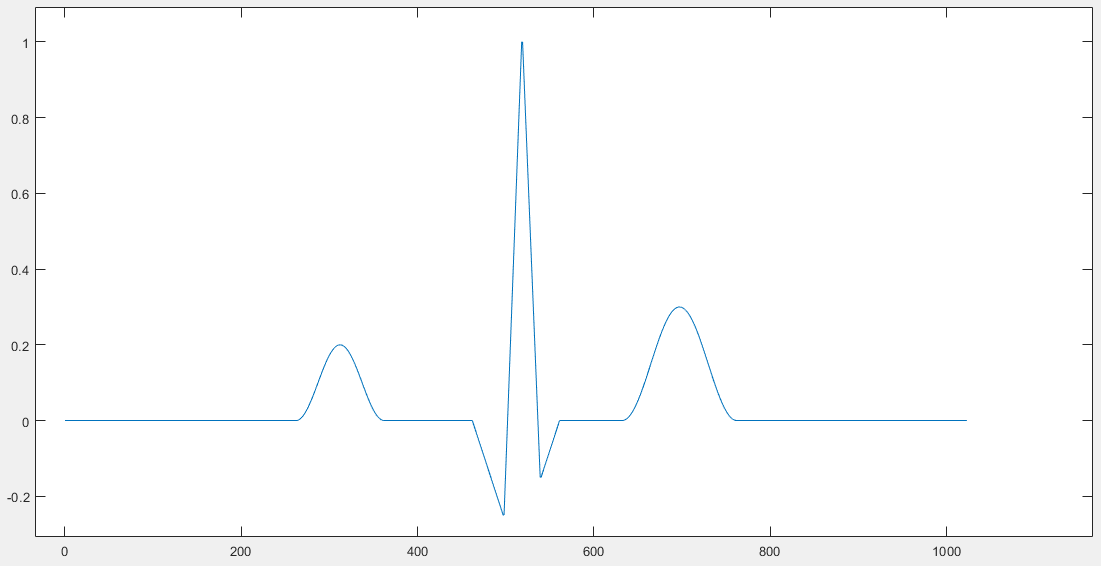
\includegraphics[width=\textwidth] {EKG_Signal.png}
	\caption{mit Matlab erstelltes künstliches EKG-Signal}
	\label{fig_Matlab EKG-Signal} 
\end{figure}

\begin{figure} [!h]
	%\centering
	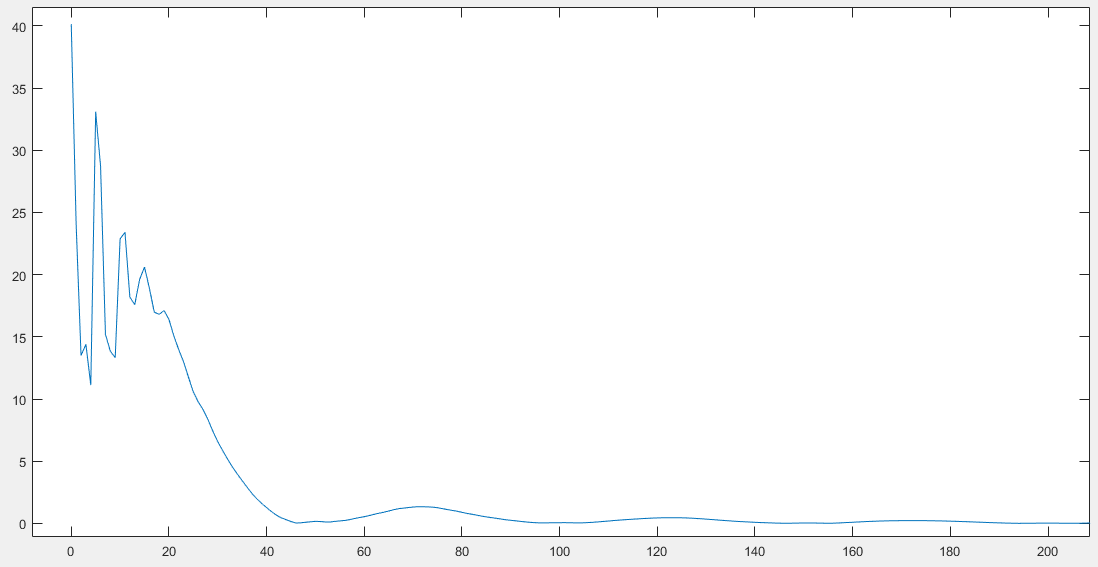
\includegraphics[width=\textwidth] {EKG_diskretes_Frequenzspektrum_Ausschnitt.png}
	\caption{Frequenzspektrum des künstlichen EKG-Signals}
	\label{fig_Matlab Frequenzspektrum} 
\end{figure}

Da das Störsignal durch Magnetfelder mit der gleichen Frequenz der Versorgungsleitungen schwingt, wird das EKG-Signal durch Kerbfilter mit einer Sperrfrequenz von \SI{50}{\hertz} gefiltert. Zur Differenzbildung der beiden Eingangskanäle wird ein Instrumentenverstärker eingesetzt. Gleichzeitig dient er zur Vorverstärkung des Signals um die Störanfälligkeit gegen elektromagnetische Felder auf dem Weg durch die Schaltung zu reduzieren. Am Ende erfolgt eine Nachverstärkung um den Arbeitsbereich und somit auch die Auflösung des ADC bestmöglich auszunutzen. Abbildung \ref{fig_Blockschaltbild Filter} zeigt die einzelnen Stufen der Filterung schematisch.

\begin{figure} [!h]
	%\centering
	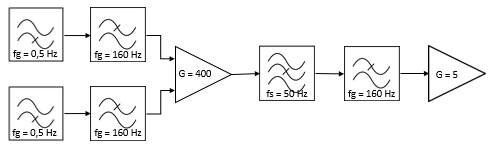
\includegraphics[width=\textwidth] {Filter Blockschaltbild.png}
	\caption{Blockschaltbild der Filterschaltung}
	\label{fig_Blockschaltbild Filter} 
\end{figure}

Wie aus Abbildung \ref{fig_Blockschaltbild} zu erkennen ist, werden zwei Versorgungsspannungen (\SI{3}{\volt}  und \SI{5}{\volt}) für die Module benötigt. Sie werden aus dem Spannungsbereich eines Lithium-Ionen-Akkus mithilfe eines LDO für \SI{3}{\volt} und eines Aufwärtswandlers für \SI{5}{\volt} erzeugt. Der Aufwärtswandler kann über einen Enable-Eingang vom Prozessor ein- oder ausgeschaltet werden, um den Stromverbrauch durch die Peripherie zu minimieren und die Akkulaufzeit zu verlängern.

Die Anzeige und Steuerung erfolgt über ein 3,2 Zoll TFT Touch Display. Es verfügt über eine serielle Schnittstelle und kommuniziert via UART mit dem Input/Ouput-Modul des Prozessors. Zur zusätzlichen Bedienung wurde ein Taster eingeplant, der zum Ein- und Ausschalten des Energiesparmodus verwendet wird. Der Buzzer dient für akustische Warnsignale bei Fehlfunktion oder einem niedrigen Ladezustand des Akkus.

Die zweite UART-Schnittstelle (Universal Asynchronous Receiver Transmitter) der CPU wird verwendet um Daten an das Bluetooth-Modul zu senden. Dieses kommuniziert dann via Bluetooth mit dem Smartphone des Benutzers, um die EKG-Daten in der App anzuzeigen.

Die Datenspeicherung erfolgt auf einer externen SD-Karte. Das Kartenmodul das zum Schreiben und Lesen der Daten verwendet wird, kommuniziert via SPI (Serial Peripheral Interface) mit dem Input/Output-Modul der CPU.


\begin{figure} [h]
	%\centering
	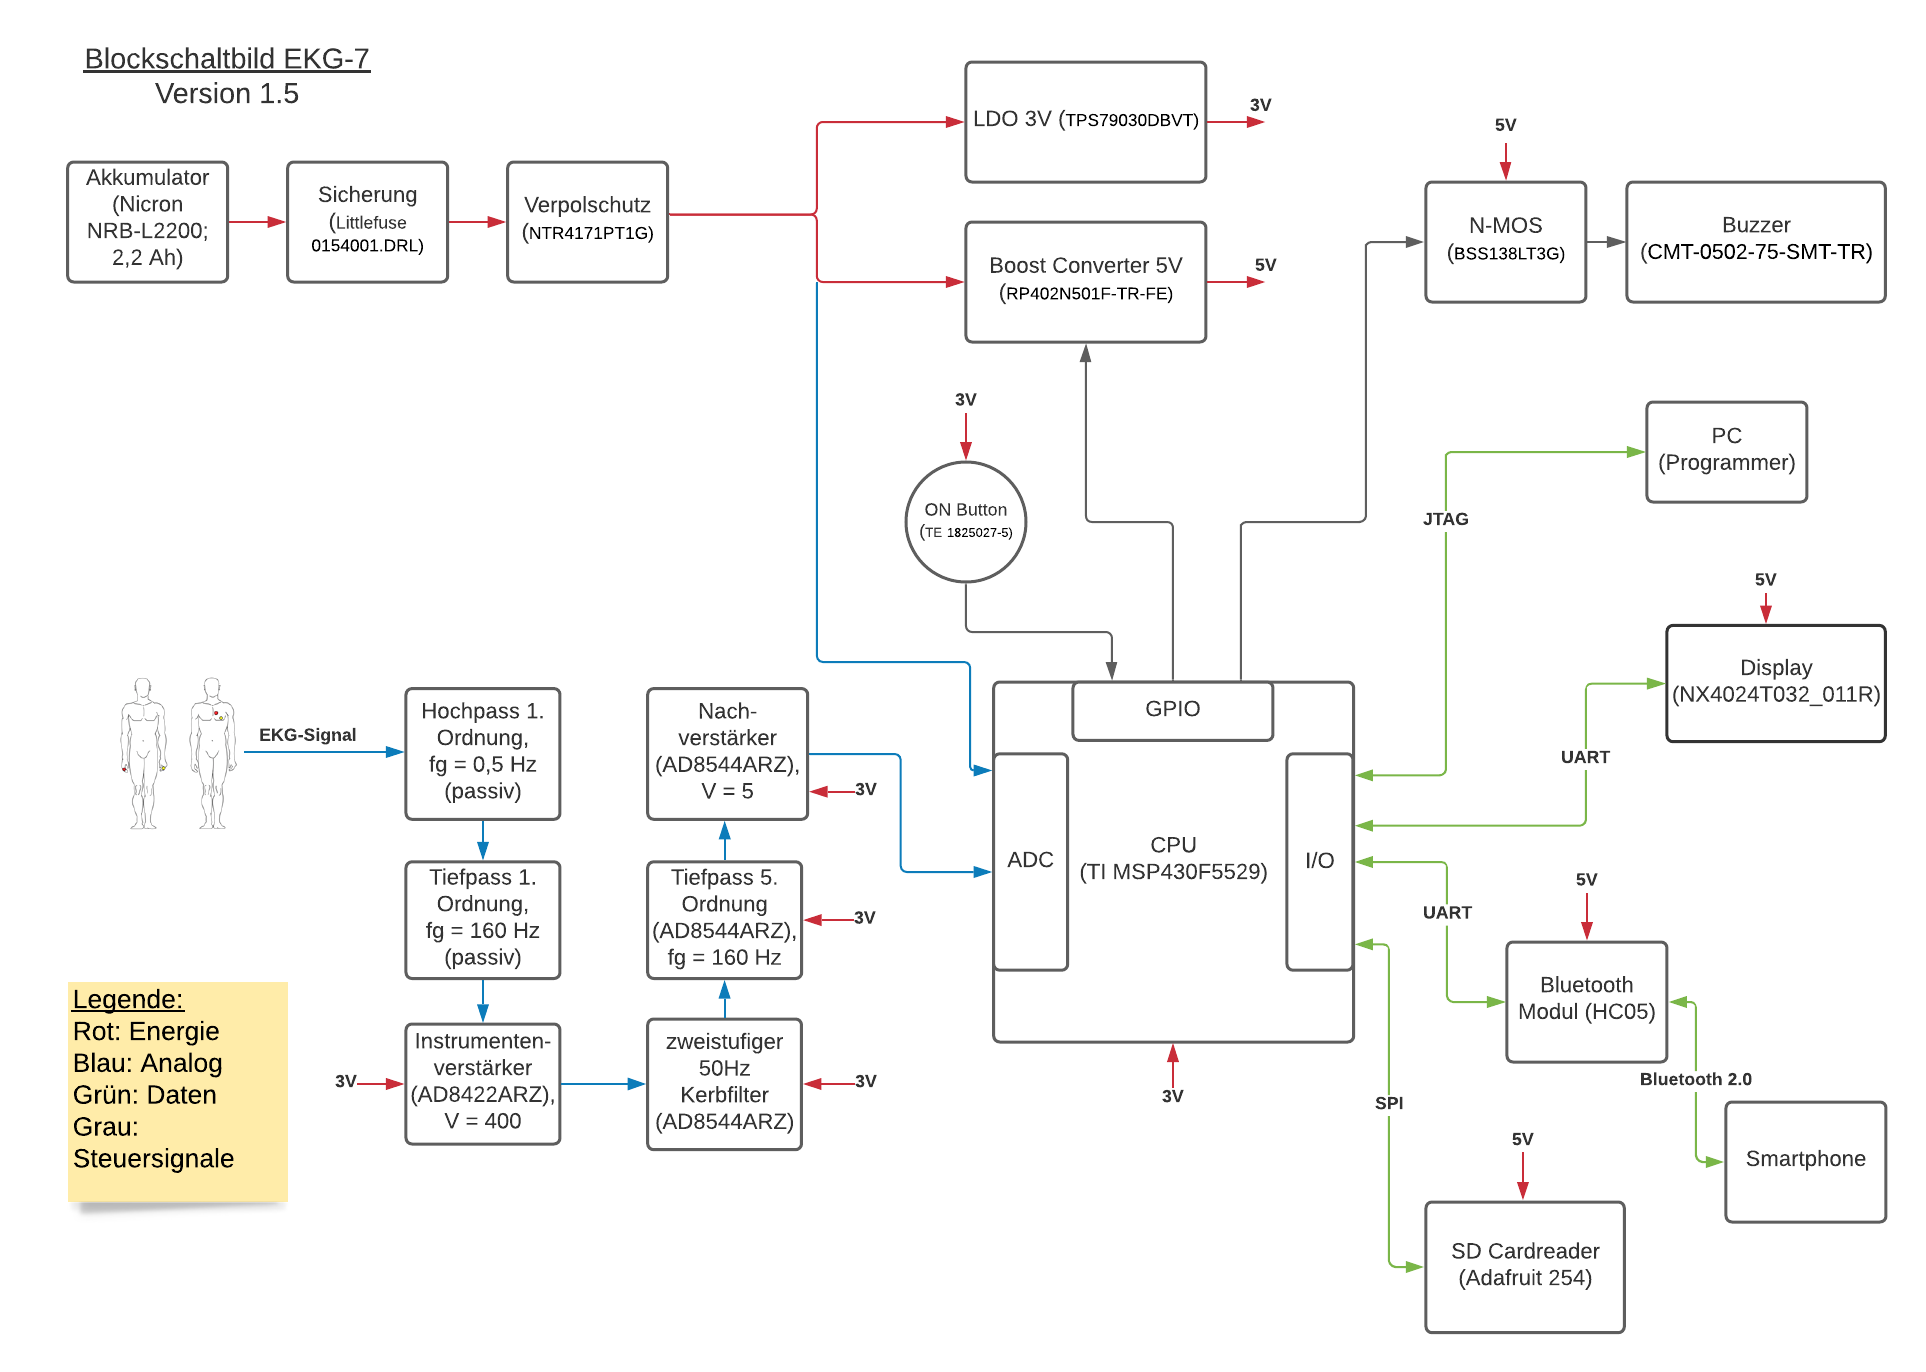
\includegraphics[width=\textwidth] {Blockschaltbild v1.5.png}
	\caption{Blockschaltbild des EKG-Geräts}
	\label{fig_Blockschaltbild} 
\end{figure}

%TODO PROJEKTGRUPPE: Konzeptionierung der jeweiligen Baugruppe; Gründe warum die jeweiligen Bauteile verwendet wurden noch hinzufügen

\subsubsection{Verwendete Software}

Für die Erstellung und Frequenzanalyse eines künstlichen EKG-Signals wurde das numerische Rechentool Matlab verwendet. Damit konnten die Grenzfrequenzen des Signals bereits ohne Labortest abgeschätzt werden. Diese Erkenntnisse wurden bei der Schaltungsentwicklung der analogen Filterschaltung mit LTSpice angewandt. Durch die Einbindung von Herstellermodellen, war die Simulation von Bauteilen möglich, ohne diese physisch zu testen. Für den Entwurf der Leiterplatine kam Altium Designer zur Anwendung. Auch hierfür bieten Hersteller Modelle für die Pinbelegung, den Footprint und 3D-Modelle an. Besonders die 3D-Modelle waren für das Gehäusedesign hilfreich um die korrekte Lage und Maße der Bauteile im Gehäuse auch optisch zu prüfen.
%TODO PROJEKTGRUPPE: weitere Software die wir verwendet haben wie Blender, Nextion Editor, CCS, Git, Android Studio etc...

\subsubsection{Verwendete Geräte}

\subsubsection{Bauteilbeschaffung und Fertigung} 

\subsubsection{Digitale Filterung}

Für die digitale Filterung des Netzbrummens wurden jeweils ein FIR- (Finite-Impuls-Response) und ein IIR- (Infinite-Impuls-Response) Filter als Bandsperren mit einer Sperrfrequenz von \SI{50} {\hertz} entworfen. Hierfür wurden die Filterkoeffizienten mit Matlab erzeugt und danach in C als eigenständige Module implementiert. Die Testung erfolgte auf dem Launchpad des MSP430 mit harmonischen Schwingungen zwischen \SI{1}{\hertz} und \SI{200}{\hertz}, einem künstlichen EKG-Signal (beides mit einer Signalquelle erzeugt) und einem echtem EKG-Signal. 

Der FIR-Filter verfügt zwar über einen linearen Phasenverlauf, erwies sich aber bei den Tests schnell als zu rechenintensiv, für die Anwendung auf dem verwendeten Prozessor. Mit ihm wurde bei einer Abtastfrequenz von \SI{250}{\hertz} lediglich eine Dämpfung von \SI{3}{\decibel} bis \SI{6}{\decibel} erreicht.

Der IIR-Filter zeigte sich im Test mit verschiedenen harmonischen Schwingungen als sehr effizient mit einer maximalen Dämpfung von \SI{150}{\decibel} bei geringem Rechenaufwand. Jedoch führte er in der Anwendung bei einem echten EKG-Signal zu einer Verschlechterung des Ausgangssignals, da er Schwingungen erzeugte, wie aus Abbildung \ref{fig_Test_IIR_Filter} zu erkennen ist. 

\begin{figure} [h]
	%\centering
	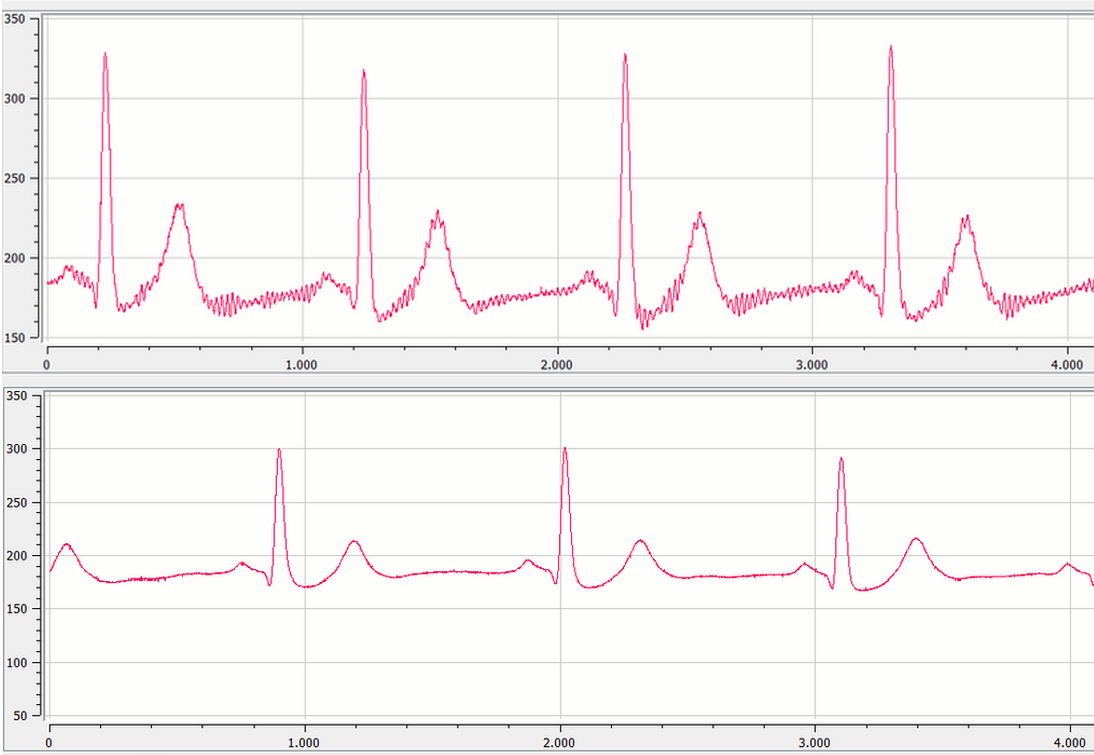
\includegraphics[width=\textwidth] {Test IIR Filter.png}
	\caption{oben: EKG-Signal mit durch IIR-Filter erzeugtes Störsignal; unten: EKG-Signal ohne IIR-Filterung}
	\label{fig_Test_IIR_Filter} 
\end{figure}
%TODO Anhang für FIR und IIR Filter



%TODO PROJEKTGRUPPE: weitere alternative Konzepte die wir ausprobiert oder in Betracht gezogen haben (zb. PMIC)

%!TEX root =  ..\ekg_7_projektbericht.tex

%Realisierung/Akkumanagement und Versorgungsspannungen

\subsection{Akkumanagement und Versorgungsspannungen}

Dieses Unterkapitel behandelt die Umsetzung der Spannungsversorgung eines mobilen EKG Gerätes.

Bei der Auswahl eines Boost-Konvertes ist vor allem auf eine hohe Effizienz des ICs sowie einen geringen Eigenverbrauch zu achten. Darüber hinaus gibt es Boost-Konverter mit einem integrierten \textit{Enable-Pin}, welcher nicht nur den IC deaktiviert, sondern auch die Last vollständig vom Eingang abkoppelt. Dies ist überaus nützlich um im Standby Strom zu sparen. Ein Konverter der all diese Anforderungen erfüllt, ist der RP402N501F-TR-FE, welcher in der Massenfertigung bereits ab 0,54 € erhältlich ist. Bei einer Effizienz von 90\% bis 94\% liefert er Ströme bis 800 mA \cite[2]{5V_DCDC_Datasheet}.
Die äußere Beschaltung dieses Wandlers beschränkt sich auf Pufferkondensatoren am Ein- und Ausgang, eine Induktivität zwischen dem Eingang und einem dedizierten Lx Pin und einem Pull-Down Widerstand am \textit{Enable-Pin}, welcher den IC auch im Fall einer deaktivieren MCU ausschaltet.

Betrachtet man den LDO ist zu beachten, dass dieser immer einen minimalen Spannungsabfall besitzt. Somit muss die Eingangsspannung größer als die Summe der gewünschten Ausgangsspannung und des Spannungsabfalls sein. Würde man z.B. eine Ausgangsspannung von 3,3 V anstreben und der LDO einen Abfall von 0,2 V besitzen, könnte man den Akku nur bis zu einer Spannung von 3,5 V entladen ohne die Ausgangsspannung zu beeinflussen. Dieser Umstand wird in Abbildung \ref{fig_DCDC_3V_plot} verdeutlicht. Deshalb wurde für das EKG-Gerät der LDO TPS79030DBVT mit einem niedrigen Spannungsabfall von 57 mV gewählt. Dieser LDO ist mit einer Restwelligkeit von 56 µV und einem Ruhestrom von 17 µA bestens zur Erfüllung der gestellten Ansprüche geeignet.

\begin{figure} [!h]
	%\centering
	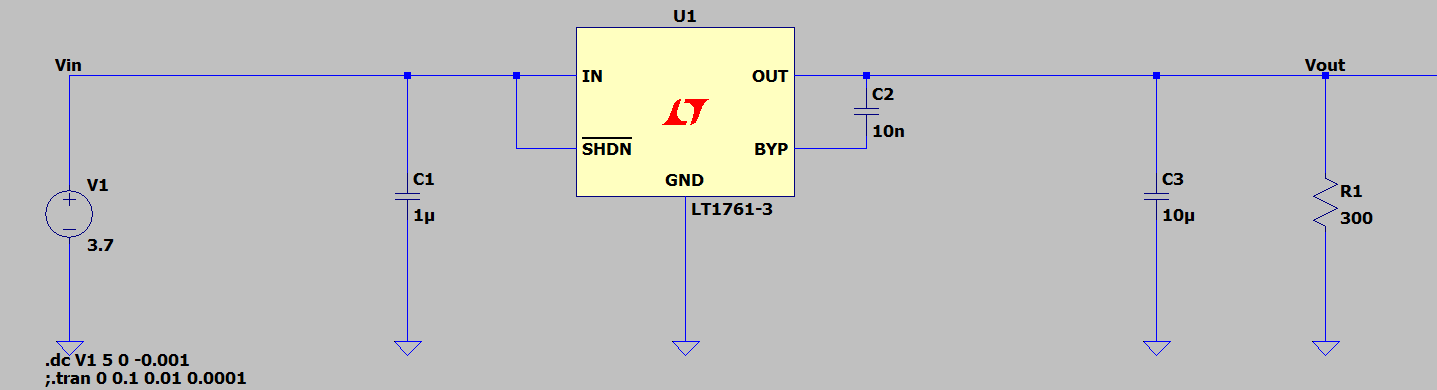
\includegraphics[width=\textwidth] {DCDC_3V_LDO_Shematic.png}
	\caption{Simulationsaufbau 3V LDO}
	\label{fig_DCDC_3V_sch} 
\end{figure}

\begin{figure} [!h]
	%\centering
	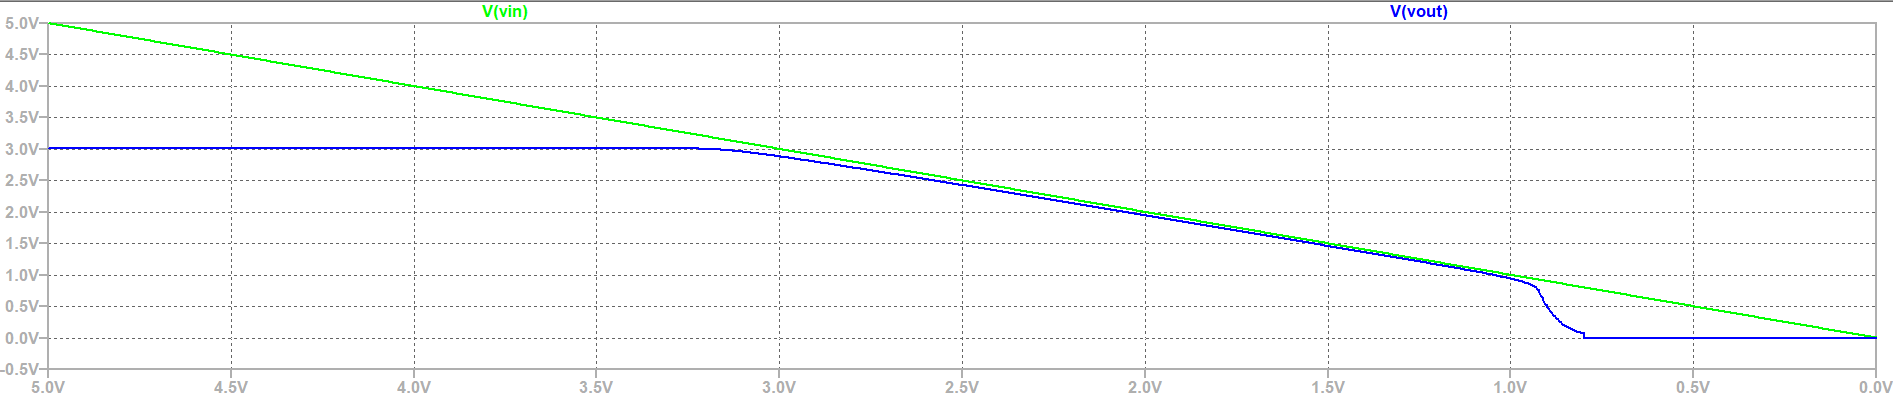
\includegraphics[width=\textwidth] {DCDC_3V_LDO_Plot.png}
	\caption{Ausgang 3V LDO mit fallender Eingangsspannung}
	\label{fig_DCDC_3V_plot} 
\end{figure}

Die Nutzung von Lithium-Ionen Zellen birgt einige Risiken. Mögliche Gefahren und getroffene Maßnahmen zur Reduktion dieser sind:

\begin{enumerate}
	\item Kurzschlüsse:	Als erste Maßnahme hierfür ist der Anschluss der Batterie als Pinkonnektor ausgeführt, wodurch sich am platinenseitigem Ende der Zuleitung eine Buchse befindet. Somit sind die Kontakte im Inneren der Buchse geschützt und können nicht durch unachtsame Handhabung kurzgeschlossen werden. Um bei Kurzschlüssen auf der Platine oder an der Peripherie den Akku zu schützen ist unmittelbar nach der Buchse eine Sicherung platziert. Hierfür wurde aus der OMNI-BLOCK Serie von Littelfuse eine 1 A-Sicherung gewählt (0154001.DRL). 
	
	\item Verpolung: Um eine Beschädigung der Schaltung durch eine verkehrt eingesetzte Batterie zu verhindern, wodurch Plus- und Minuspol vertauscht wären, ist ein Verpolschutz durch einen PMOS vorhanden. Der \textit{Drain}-Anschluss liegt hierbei an der Batterie während der \textit{Source}-Anschluss dem Rest der Schaltung zugewandt ist. Dadurch ist bei korrekter Polung die \textit{Body}-Diode von \textit{Drain} nach \textit{Source} leitend. Das \textit{Gate} ist über einen Widerstand mit der Masse verbunden, wodurch im Normalbetrieb eine negative \textit{Gate-Source} Spannung anliegt und den Transistor komplett durchsteuert. Im Fall einer Verpolung ist die \textit{Body}-Diode nicht leitend und es entsteht keine Potentialdifferenz zwischen \textit{Gate} und \textit{Source}. Der FET sperrt und die Schaltung ist geschützt.

	\item Überspannung:	Überspannungen z.B. durch eine elektrostatische Entladung (ESD) beim wechseln der Batterie können der Schaltung Schaden zufügen. Zur Prävention ist am Spannungeingang eine bidirektionale \textit{Transient Voltage Suppressor} (TVS) Diode verbaut, welche Spannungen über 9V erdet.
	
	\item Tiefenentladung: Eine Entladung auf Spannungen außerhalb der Spezifikation des Akkus können zu dessen Zerstörung führen. Aus diesem Grund wird fortwährend die aktuelle Akkuspannung des Geräts durch die MCU gemessen und der Nutzer bei Handlungsbedarf darauf hingewiesen. Zusätzlich wird ein Akku mit integrierter Schutzbeschaltung verwendet, welche ebenso einen Tiefentladungsschutz enthält.
\end{enumerate}



%EKG-7 Realisierung/Display und UI

\subsection{Display und Benutzeroberfläche}

Dieses Unterkapitel behandelt die Auswahl des Displays und die Programmierung der Benutzeroberfläche.

\subsubsection{Auswahl des Displays}
Gesteuert wird das EKG-Gerät durch das NX4024T032. Dabei handelt es sich um ein TFT Touch-Display der Firma Nextion. Das Display ist 3,2 Zoll groß und weist eine Auflösung von 400x240 Pixel auf. Betrieben wird das Display mit 5 V und verbraucht bei maximaler Helligkeit 85 mA. Verbunden wird das Display via UART mit einer Baudrate von 115200 $s^{-1}$.

\subsubsection{Programmierung der Benutzeroberfläche}
Der erste Schritt der Displayprogrammierung ist die Initialisierung. In diesem Schritt wird die Baudrate von 115200 $s^{-1}$ und die \textit{„Tap-to-wake“} Funktion integriert. Das Display schaltet sich je nachdem, auf welcher Seite man sich befindet, nach 30 bis 180 Sekunden in den Schlafmodus. Durch einmaliges Antippen auf das Display wird es wieder aufgeweckt.

Der Nextion-Editor verfügt über ein weites Spektrum an Werkzeugen von denen folgende im Projekt verwendet werden:
\begin{itemize}
    \item \textit{Text}: Für die Beschreibung der Funktionen und Anleitung
    \item \textit{Number}: Variablen für den \textit{Timer}, Ladestand und Herzfrequenz
    \item \textit{Button}: Zum Seitenwechsel und senden der \textit{Interrupts} an die MCU
    \item \textit{Waveform}: Für den EKG-Kurvenverlauf
    \item \textit{Slider}: Einstellung der Helligkeit
    \item \textit{Timer}: Befehle, die regelmäßig ausgeführt werden
\end{itemize}

Aufgebaut ist die Benutzeroberfläche aus verschiedenen Seiten. Nach dem Einschalten des EKG-Gerätes gelangt man auf die Startseite (siehe Abbildung \ref{fig. EKG-Startseite}). Hier ist in der oberen rechten Ecke die Peripherie zu sehen. Der Akkustand wird in Prozent angegeben und die Verbindung zur SD-Karte und zum Bluetooth-Modul überprüft. Bei einem blauen Symbol besteht eine Verbindung und bei einem grauen Symbol ist das Modul getrennt. Alle Symbole die auf dem Display vorzufinden sind, wurden aus Vorlagen an das gesamte Erscheinungsbild der Oberfläche angepasst.
\begin{figure} [!h]
	\centering
	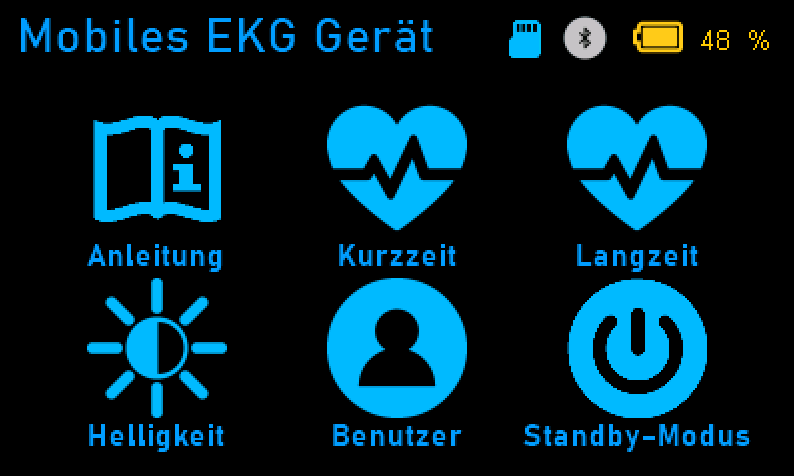
\includegraphics[width=10cm] {ECG_Homescreen.png}
	\caption{Startseite des EKG-Gerätes}
    \label{fig. EKG-Startseite}
\end{figure}

Die sechs Symbole in der Mitte des Displays sind \textit{Buttons}, mit denen zwischen den Seiten gewechselt wird. In der Anleitung werden allgemeine Einstellungen erklärt, wie die Elektroden am Patienten anzubringen sind und welche Funktionen ein Kurzzeit- und Langzeit-EKG bietet. Beim Kurzzeit-EKG erfolgt eine zweiminütige Aufzeichnung, welche in Echtzeit auf dem Display nachverfolgt werden kann. Beim Langzeit-EKG erfolgt die EKG-Aufnahme für 24 Stunden. Die Helligkeit des Displays kann mithilfe eines Schiebereglers eingestellt werden. Optional kann ein Benutzer ausgewählt werden. Dieser Benutzer erscheint dann auf der erstellten CSV-Datei der SD-Karte. Der \textit{Standby-Modus} versetzt das Display beim Drücken in den \textit{Sleep-Modus}.

Während der Nutzung des EKG-Gerätes sind diverse Sicherheitsabfragen auf dem Display vorzufinden, wenn:
\begin{enumerate}
    \item bereits eine Aufnahme läuft und eine Andere gestartet wird.
    \item eine Aufnahme mit dem Stopp-Befehl abgebrochen wird.
    \item die SD-Karte entfernt wird oder beim Anschaltvorgang fehlt.
    \item der Ladestand des Akkus bei einer Langzeit-Aufnahme kleiner als 80 \% ist.
    \item Verdacht auf Bradykardie oder Tachykardie besteht.
\end{enumerate}

Die Herzfrequenz wird während einer Kurzzeit-Aufnahme kontinuierlich berechnet. Da es sich bei diesem Projekt um ein Ruhe-EKG handelt, sollte die Herzfrequenz im Ruhebereich liegen. Im Fall von Bradykardie oder Tachykardie wird der Patient auf dem Display visuell gewarnt.



%EKG-7 Realisierung/Prozessoreinheit

\subsection{Prozessoreinheit}

Dieses Kapitel gibt eine ausführliche Beschreibung zur Software des Projektes und deren Entwicklung. Zuerst wird der Begriff \textit{State Machine} im Allgemeinen beschrieben. Anschließend wird auf die Implementierung der \textit{State Machine} im Projekt mit der Beschreibung jedes Zustandes eingegangen, sowie auf essenzielle Module und Funktionsprinzipien.  

\subsubsection{State Machine}

Eine \textit{State Machine} ist ein Verhaltensmodell der Softwareentwicklung mit einer endlichen Anzahl von Zuständen. Zwischen diesen Zuständen kann gemäß der Programmlogik oder der Eingangsdaten gewechselt werden. \cite{State_Machine}

Eine \textit{State Machine} hat in der Regel einen Initialisierungszustand, in dem die Programmmodule gestartet werden. Der folgende Programmablauf ist von dem Initialisierungszustand abhängig. Nach einer erfolgreichen Initialisierung wird beispielsweise der reguläre Programmablauf fortgeführt. Sollte es bei der Initialisierung zu Fehlern kommen, wird ein Zustand eingenommen indem z.B. mögliche Fehlerursachen angezeigt oder das komplette System abgeschaltet wird. Die Überwachung von Fehlfunktionen findet auch in allen anderen Zuständen statt.

\subsubsection{Zustände der \textit{State Machine}}

In diesem Projekt sind sechs verschiedene Zustände für das EKG-Gerät entwickelt, sowie eine regelmäßige Abfrage der globalen Flags, die jede Sekunde stattfindet. Die Zustände der \textit{State Machine} sind: 
\begin{itemize}
    \item Initialisierung – SYS\_INIT
    \item Leerlauf – IDLE\_STATE
    \item Aufnahme des Kurzzeit-EKG – ECG\_SHORT
    \item Aufnahme des Langzeit-EKG – ECG\_LONG
    \item Stromsparmodus – ENERGY\_SAVING\_MODE
    \item Wakeup Modus – SYS\_WAKEUP
\end{itemize} 
Aus dem Bild ist die Funktionsweise der \textit{State Machine} zu entnehmen. Auf den genauen Ablaub wird in der Beschreibung der einzelnen Zustände eingegangen.
\begin{figure} [!h]
    \centering
    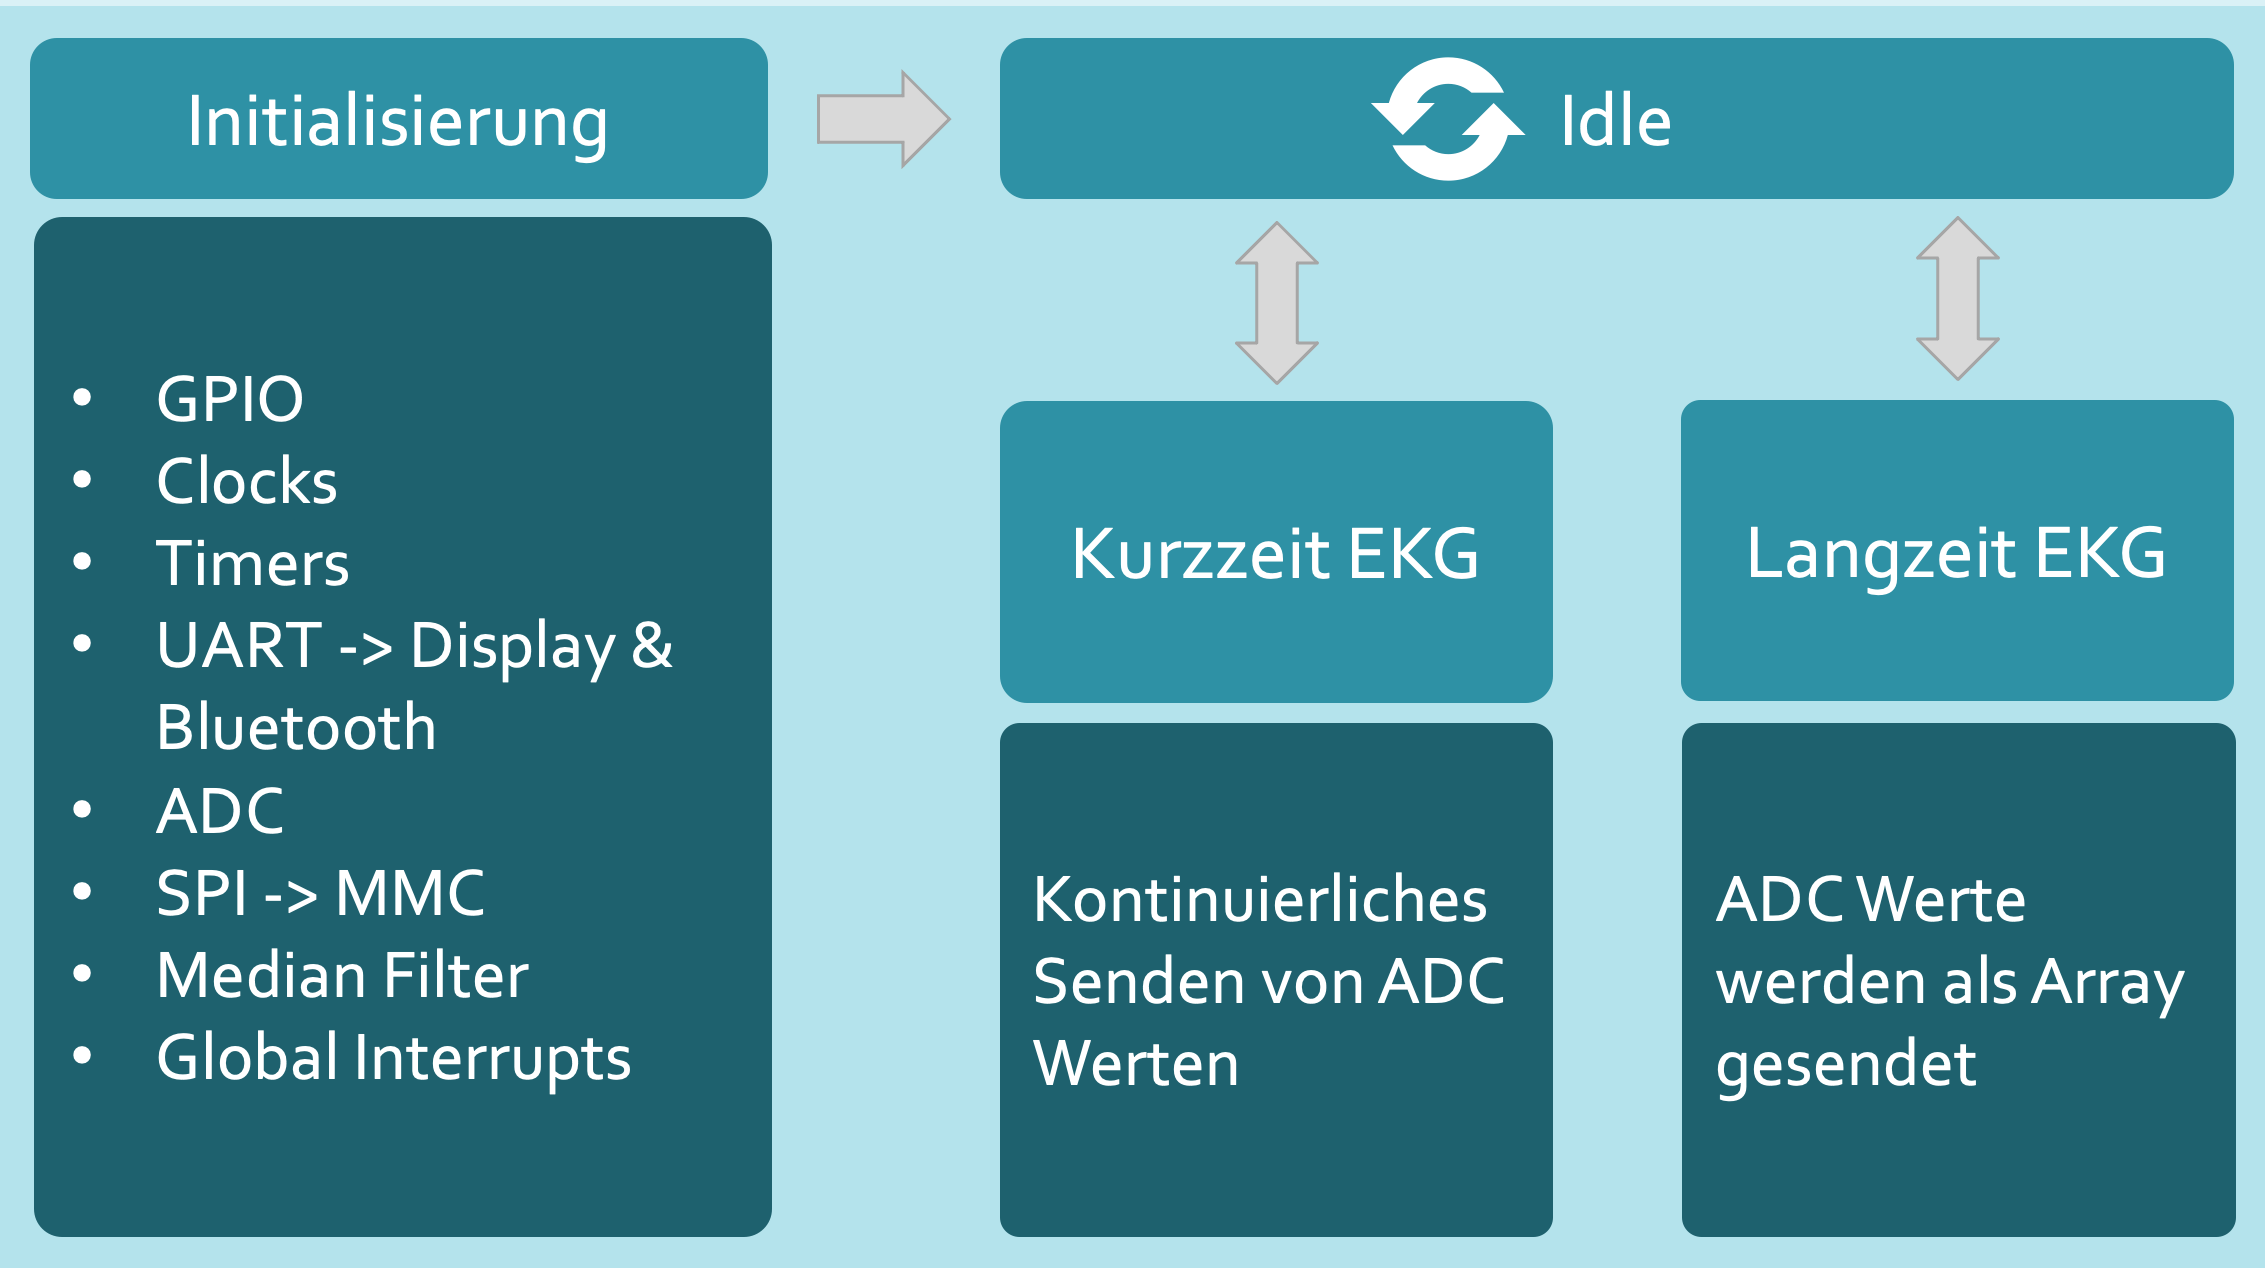
\includegraphics[width=12cm] {State Machine.png}
    \caption{\textit{State Machine} des EKG7}
\end{figure}

\subsubsection{Globale Flags}

Für das Anzeigen diverser Zustände sind in der Software globale \textit{Flags} implementiert. Die \textit{Flags} können folgende Ereignisse widerspiegeln:
\begin{itemize}
    \item Auftreten eines \textit{Interrupts}
    \item Eingang von Daten
    \item Aktueller Zustand der \textit{State Machine}
    \item Betätigen des \textit{Power-Buttons}
    \item Zustände der Module (z.B. aktiv / inaktiv)
    \item \textit{Timer-Interrupt}
    \item Zustand der Bluetooth-Verbindung
    \item Verbindung mit SD-Karte
\end{itemize} 

\subsubsection{Interrupts}

Ein Interrupt ist ein Signal an die MCU, das hardware- oder softwareseitig auftritt und eine sofortige Reaktion der MCU benötigt. Der normale Programmablauf wird dabei gestoppt und zunächst die Befehle der ISR ausgeführt. Nach dem Abarbeiten eines \textit{Interrupts} kehrt die MCU zurück zum normalen Programmablauf. \cite{Interrupt1} \cite{Interrupt2} 
In dem Projekt werden \textit{Interrupts} für folgende Module verwendet:
\begin{itemize}
    \item GPIO – beim Betätigen der Taste am Gehäuse, Ein- und Ausschalten des Bluetooth Moduls und Einsetzen bzw. Entfernen der SD-Karte
    \item Timer – es treten drei \textit{Interrupts} mit jeweils 1 Hz, 250 Hz und 1 kHz Frequenz auf
    \item UART – beim Empfang von Befehlen vom Display
    \item ADC – beim Empfang von EKG-Signalen und Akkuspannung
\end{itemize} 

\subsubsection{Initialisierung}

Initialisierung oder SYS\_INIT ist der Anfangszustand der MCU nach dem Einschalten. Dieser Zustand ruft die Initialisierungsfunktion aller verwendeten Modulen auf und wird danach verlassen. 

%Hier folgt die Reihenfolge der Module, die im Programm initialisiert werden:
%\begin{itemize}

 %   \item Clocks – ;
 %   \item Timer – 
 %   \item UART – Schnittstelle für Display- und Bluetooth-Verbindung;
 %   \item ADC – Digitalisierung der analogen Signale;
 %   \item SPI – Schnittstelle für Verbindung mit SD-Kartenmodul;
 %   \item FAT – File Allocation Table ist die Dateizuordnungstabelle bzw. ein Dateisystem für die Datenübertragung auf SD-Karte;
 %   \item UART-BT – Kommunikation der MCU mit dem Bluetooth-Modul;
 %   \item Median Filter – Filterung der Artefakte bei der Herzfrequenzberechnung;
 %   \item Globle Interrupts – Freischalten der globalen Interrupts.
%\end{itemize}

Im Folgenden wird eine detaillierte Beschreibung von den zu initialisierenden Modulen aufgelistet:
\begin{enumerate}
    \item Watchdog Timer: Ist dem Totmann-Schalter ähnlich. Die MCU wird zurückgesetzt, wenn das Programm ihn nicht explizit ausschaltet \cite{Watchdog_Timer}
    \item GPIO: General Purpose Input Output ist ein Modul, das die vorhandenen Pins als Inputs oder Outputs initialisiert. Da ihre Funktionalität in aderen Modulen verwendet wird, müssen sie als erstes initialisiert werden. Es werden folgende GPIO-Pins initialisiert:
    \begin{itemize}
        \item LEDs auf der Platine
        \item Buzzer
        \item 5 V-DC/DC enable
        \item Gehäusetaste
        \item Bluetooth-Verbindungszustand
        \item \textit{Card Detect} Pin für das SD-Kartenmodul
    \end{itemize}
    \item Clocks: Es werden drei \textit{Clocks}  für den Mikrocontroller initialisiert. MCLK und SMCLK weisen eine Frequenz von 20 MHz auf. ACLK ist mit einer Frequenz von 32 kHz initialisiert.
    MCLK wird als Taktquelle für die MCU verwendet. SMCLK ist ein Hochfrequenztakt und wird für Peripheriemodule verwendet. ACLK wird für Peripheriemodule verwendet, die einen niederfrequenten Takt benötigen.
    \item Timer: Die \textit{Timer} lösen in gewissen Zeitintervalen \textit{Interrupts} aus. Im Code sind drei \textit{Timer} initialisiert. \textit{Timer} A0 bezieht seinen Takt von SMCLK und hat eine Frequenz von 1 kHz. \textit{Timer} A1 hat ACLK als Taktgeber und wird mit einer Frequenz von 1 Hz aufgerufen. Timer A2 ist an SMCLK gebunden und weist eine Frequenz von 250 Hz auf. Die drei \textit{Timer} funktionieren unabhängig voneinander und haben ihre eigene ISR.
    \item UART Display: Bei der Initialisierung der UART Verbindung zum Display, werden zunächst die Input- (RX) und Output- (TX) Pins festgelegt. Die Frequenz der MCU beträgt 20 MHz und als Baudrate wurde 115200 $s^{-1}$ gewählt. Damit eine Verbindung der beiden Module hergestellt werden kann, muss die Baudrate sowohl beim Display als auch bei der MCU einprogrammiert werden.\\
    Befehle vom Display an die MCU werden mittels \textit{Interrupts} realisiert. Das Display sendet eine Folge zwischen vier und sieben Bytes. Sobald die MCU eine gesendete Byte-Folge erkennt, werden in einem \textit{Interrupt Flags} gesetzt. Anhand dieser \textit{Flags} werden im späteren Verlauf gewisse Funktion auf der MCU aufgerufen.\\
    Bei Befehlen, die von der MCU an das Display gesendet werden, wird im Wesentlichen mit drei Funktionen gearbeitet. Bei der ersten Funktion wird ein Befehl mit der entsprechenden Variablen als \textit{String} (z.B. „page0.akku.val“) an das Display gesendet. Mit der zweiten Funktion wird der dazugehörende Wert, zum Beispiel \textit{akku\_percentage}, von einem \textit{Integer} Wert in einen \textit{String} umgewandelt und anschließend an das Display sendet. Um einen Befehl abzuschließen, erwartet das Display drei Bytes mit dem Inhalt „0xFF“ am Ende. Diese drei Bytes werden in der dritten UART-Funktion an das Display gesendet.
    \item UART Bluetooth-Modul: Das verwendete Bluetooth-Modul HC-05 wird über UART angesprochen, wobei die Baudrate 38400 $s^{-1}$ beträgt. Seitens der MCU wird das Hardware-Modul USCI\_A1 verwendet, welches mit Ausnahme der Basisadresse identisch zu USCI\_A0 bzw. Display initialisiert wird.\\
    Um beim Versenden der Nachrichten keine Verzögerung oder zusätzliche CPU Last zu verursachen, wird \textit{Direct Memory Access} (DMA) verwendet. Das DMA-Modul kann automatische Daten im Hintergrund in das TX Register des UART Moduls kopieren. Hierfür wird nach jedem Trigger die Information byteweise übertragen. Als Trigger wird das \textit{Interrupt Flag} UCA1TXIFG gewählt, welches immer dann aktiv ist, wenn das UART Modul bereit ist ein weiteres Byte zu senden.\\
    Damit ein ganzer \textit{String} verschickt werden kann, inktementiert das DMA Modul die Quelladresse nach jedem versendeten Byte. Somit wird nach Aktivierung des Moduls durch setzen des DMA-Enable-Bits ein kompletter String im Hintergrund Byte für Byte versendet, bis die vorgegebene Datengröße abgearbeitet ist und das Enable-Bit automatisch zurückgesetzt wird. Die CPU selbst wird dabei jeweils nur für zwei Takte durch das DMA Modul unterbrochen und muss nicht auf den Abschluss jedes Sendevorgangs warten.
    \item ADC: Danach wird das ADC Modul initialisiert und die beiden Pins für die EKG-Aufnahme und Akkuüberwachung konfiguriert. Als positive Referenzspannungsquelle wird AVCC (3V) für beide ADC Kanäle eingestellt. Negative Referenzspannungsquelle ist AVSS, was dem Massepotential auf der Platine entspricht. Beide Kanäle werden mit ACLK betrieben. Zum Schluss wird der \textit{Interrupt} für dieses Modul aktiviert.
    \item SPI: Die SPI Schnittstelle dient zur Kommunikation mit dem SD-Kartenmodul und wird mit der SMCLK betrieben. Nach dem die gewünschte Frequenz eingestellt wurde, werden die \textit{Interrupts} freigeschaltet, das \textit{Chip Select} Signal an den \textit{Slave} gesendet und der TX Buffer aktiviert.
    \item FAT: Als Kommunikationsprotokoll für FAT, wird die Schnittstelle SPI verwendet. Das FAT-Modul ist für die Initialisierung der SD-Karte verantwortlich. Dafür wird in diesem Projekt eine \textit{Open Source Library} verwendet. \cite{FatFs_Lib} \cite{FatFs_Entwickler} 
    \item Medianfilter: Der Medianfilter dient dazu, Ausreißer (verursacht durch Bewegungsartefakte des Anwenders) der berechneten Herzfrequenz herauszufiltern. In der Initialisierung wird ein Array mit elf Elementen angelegt, dass als Speicher des Filters dient. Aus diesem Speicher wird nach jeder neuen Pulsberechnung der Median gebildet und ans Display gesendet. Im Gegensatz zu einem Mittelwertfilter haben vereinzelte Ausreißer keinen Einfluss auf das Ergebnis.
\end{enumerate}

\subsubsection{Idle State}

Direkt nach dem Initialisierungsvorgang der MCU wechselt sie in den \textit{IDLE\_STATE} (Leerlauf des Programms). 
Hier wird kontinuierlich abgefragt, ob der Marker für ein Kurz- oder Langzeit-EKG gesetzt ist. Der Marker wird im \textit{Interrupt} gesetzt, der ausgelöst wird nachdem der Benutzer die Aufnahme des EKG startet.
Sobald der Benutzer den Befehl gibt, wird eine CSV Datei auf der SD-Karte erstellt und der Zustand der \textit{State Machine} wechselt entsprechend der gewünschten Aufnahmemethode.

\subsubsection{Kurzzeit-EKG}

Im Falle einer Kurzzeit-Aufnahme startet man das EKG auf dem Display im Unterpunkt „Kurzzeit EKG“. Sobald dieser Befehl ausgeführt wurde, läuft die Aufnahme samt Speicherung für zwei Minuten automatisch ab.\\
Die EKG-Aufnahme wird kontinuierlich durchgeführt. Das heißt die ADC Werte werden direkt an das Display und an die SD-Karte übertragen, ohne vorher zwischengespeichert zu werden. Nachdem die MCU in den Zustand \textit{ECG\_SHORT} wechselt, wird als erstes ein \textit{Timer} auf dem Display gestartet. Der \textit{Timer} zeigt an, wie lange die EKG-Aufnahme bereits läuft. Zunächst wird auf eine 250 Hz \textit{Flag} gewartet. Sobald die \textit{Flag} ungleich Null ist, wird ein ADC Wert aufgenommen und die \textit{Flag} zurückgesetzt. Der aufgenommene Wert wird an das Display gesendet und mit einer Zeitsignatur auf die SD-Karte gespeichert.\\
Es wird stets kontrolliert, ob während der Aufnahme ein Langzeit-EKG gestartet wird. Sollte dies geschehen, wird eine Warnung auf dem Display angezeigt und der Vorgang verhindert.\\
Nach dem Ende der Aufnahme wird die \textit{Flag} für das Kurzzeit-EKG und der Display-\textit{Timer} zurückgesetzt, die Datei auf der SD-Karte gespeichert und die MCU gelangt wieder in den \textit{IDLE\_STATE}. Um das EKG vorzeitig abzubrechen, kann der Stopp-Button des Displays betätigt werden. Der Abbruch muss dann in einer Sicherheitsabfrage erneut bestätigt werden. Erst danach wird die Aufnahme gestoppt. Ansonsten läuft die Aufnahme bis zur Vollendung der zwei Minuten weiter.

\begin{figure} [!h]
	%\centering
	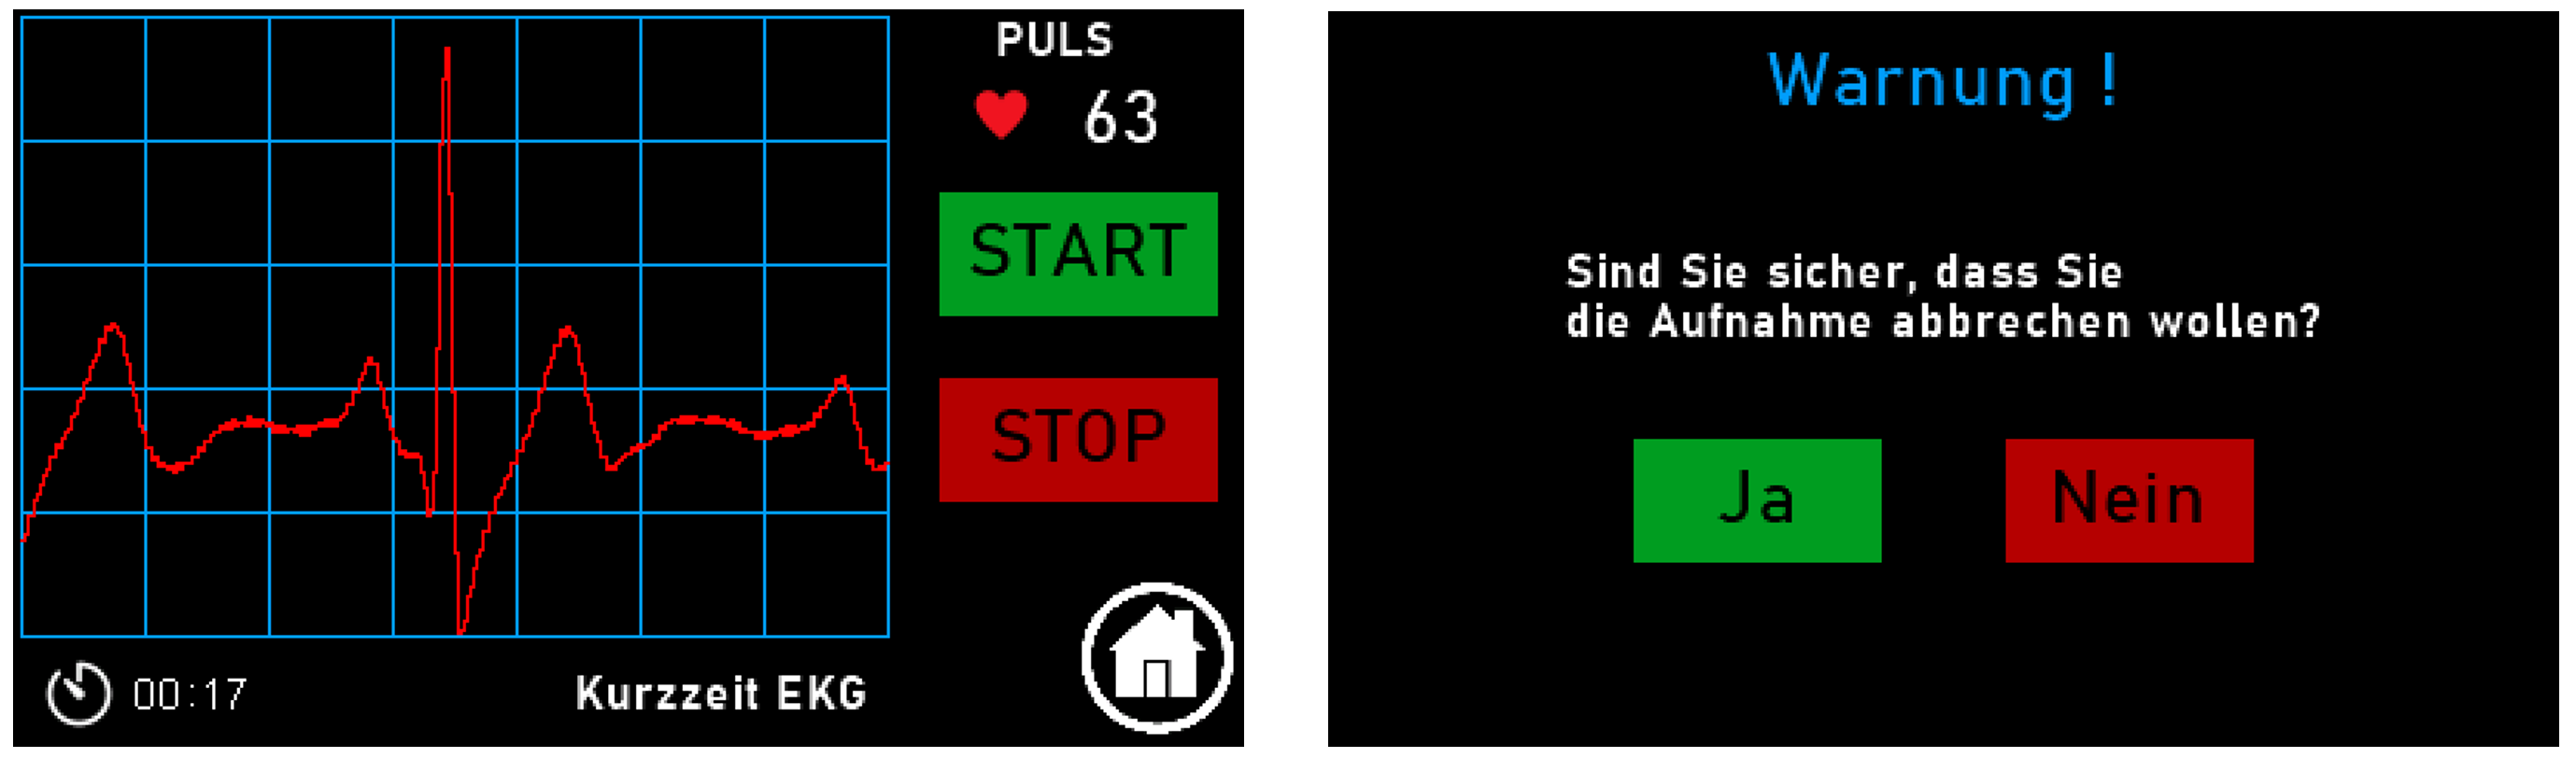
\includegraphics[width=\textwidth] {Short ECG.png}
	\caption{Display UI einer Kurzzeit-Aufnahme}
\end{figure}

Im Kurzzeitmodus wird zudem kontinuierlich die Herzfrequenz gemessen und an das Display gesendet. Hierfür werden über einen Schwellwert die R-Zacken des Signals detektiert und die Anzahl der Werte zwischen diesen gezählt.

$$ Pulsfrequenz = \frac{\textit{Samples pro Minute}}{\textit{Samples zwischen zwei R-Zacken}} $$

Der Schwellwert wird permanent durch das Maximum und Minimum der vergangenen Signalperiode angepasst, um auf Schwankungen des Signals zu reagieren.

$$ Schwellwert = Minimum + 0,8 \cdot (Maximum - Minimum) $$

\subsubsection{Langzeit-EKG}

Während der Langzeit-Aufnahme werden die Daten auf der MCU gespeichert und alle vier Sekunden blockweise an die SD-Karte gesendet. Gestartet wird ebenfalls durch einen Start-Befehl auf dem Display. Hier ist jedoch zu beachten, dass der Ladestand beim Start mindestens 80 \% aufweisen muss, um eine EKG-Aufnahme über 24 Stunden zu gewährleisten. Wie im Kurzzeit-Modus kann der Benutzer den Kurvenverlauf und die Aufnahmedauer am Display ansehen. 

Durch Betätigen des Tasters wird der Energiesparmodus aktiviert. Die Logik des Stromsparmodus enthält eine weitere \textit{State Machine} mit drei Zuständen. Die State Machine ist mit einer switch-Anweisung realisiert. Die drei Zustände sind: normaler Zustand \textit{(MODE\_NORMAL)}, 5V Peripherie an \textit{(MODE\_5V\_ON)} und 5V Peripherie aus \textit{(MODE\_5V\_OFF)}. Das Funktionsprinzip des Energiesparmodus ist auf dem Bild zu sehen.

\begin{figure} [!h]
    \centering
    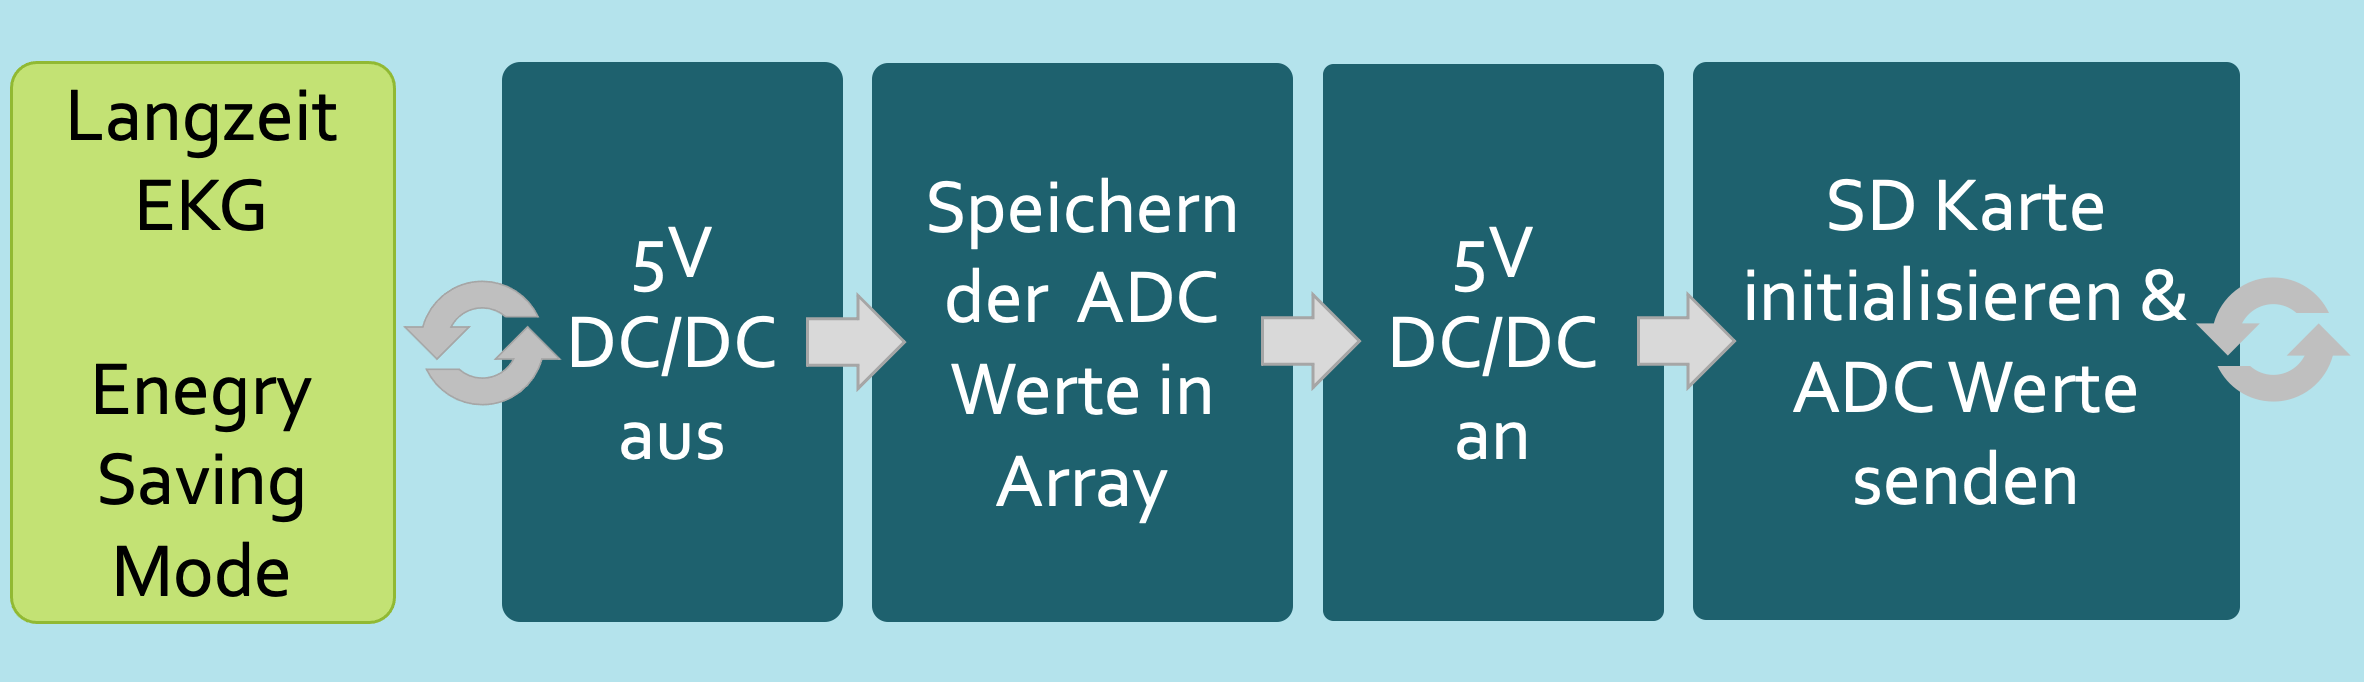
\includegraphics[width=12cm] {Langzeit EKG Energy Saving.png}
    \caption{Energy Saving Mode während Langzeit-EKG}
\end{figure}

Im normalen Zustand bleibt die ganze 5 V-Peripherie angeschaltet. Der Kurvenverlauf ist auf dem Display zu sehen. Der einzige Unterschied ist das Schreiben auf die SD-Karte. Hierfür werden zwei Arrays (\textit{Main} und \textit{Redundant Storage}) mit jeweils 1000 Werten genutzt. Da der ADC an den 250 Hz-Timer gebunden ist, wird das \textit{Main Storage} Array innerhalb von vier Sekunden gefüllt. Ist das voll, werden die Werte in das \textit{Redundant Storage} Array kopiert, aus welchem dann auf die SD-Karte geschrieben wird. Somit kann das \textit{Main Storage} Array zeitgleich wieder überschrieben werden und es gehen keine Werte durch den Schreibvorgang verloren. Nachdem das Senden beendet ist, wiederholt sich der ganze Vorgang.\\
Wenn der Taster betätigt wird, geht die MCU aus dem Zustand \textit{MODE\_NORMAL} in den \textit{MODE\_5V\_OFF}. In diesem Zustand wird die 5 V-Peripherie abgeschaltet. Der Zustand kann verlassen werden, wenn entweder \textit{Main Storage} voll ist oder der Taster erneut betätigt wird.\\
Wenn das Main Storage Array voll ist, geht die MCU in den Zustand \textit{MODE\_5V\_ON}, in dem die 5 V-Peripherie wieder versorgt wird. Im nächsten Schritt wird die SD-Karte initialisiert und das bereits kopierte \textit{Redundant Storage} auf die SD-Karte geschrieben. Danach geht die MCU in den Zustand \textit{MODE\_5V\_OFF} und der Vorgang wird wiederholt.\\
Wechselt der Benutzer durch Betätigen des Tasters wieder in den \textit{MODE\_NORMAL}, kann die Aufnahme wie im Kurzzeit-EKG abgebrochen werden. Hierbei erfolgt eine Sicherheitsabfrage, anderenfalls läuft die Aufnahme automatisch für 24 Stunden. Die MCU gelangt danach zurück in den \textit{Idle State}.

\subsubsection{Energy Saving Mode und Wakeup Mode}

Um die Batterielaufzeit bei einer Lagerung des Gerätes zu verlängern, verfügt es über einen Energiesparmodus. Wenn das Gerät eingeschaltet ist und sich im \textit{IDLE\_STATE} befindet, kann der Taster am Gehäuse gedrückt werden. Dabei wird in den Zustand \textit{ENERGY\_SAVING\_MODE} gewechselt. Dieser schaltet den 5 V-DC/DC und die damit verbundene Peripherie ab. Beim Ausschalten ist ein akustisches Signal des Buzzers zu hören. Die Überwachung des SD-Kartenstatus läuft über 3 V. Daher ist diese selbst im \textit{ENERGY\_SAVING\_MODE} vorhanden. Sollte die SD-Karte währenddessen entfernt werden, wird eine SD-\textit{Flag} im GPIO gesetzt.
Wenn im Energiesparmodus der Taster am Gehäuse erneut betätigt wird, gelangt man in den Zustand \textit{SYS\_WAKEUP}. In diesem Zustand wird die 5 V-Peripherie wieder angeschaltet und das akustische Signal des Buzzers ist zu hören. Sollte die SD-Karte während dem Energiesparmodus entfernt worden sein, wird der Benutzer auf dem Display darauf hingewiesen. Sollte die SD-Karte nun erneut eingesteckt werden, erfolgt eine Initialisierung und das SD-Kartensymbol auf dem Display wird aktualisiert.
Das EKG-Gerät befindet sich anschließend wieder im \textit{IDLE\_STATE}.

Die Logik wird Anhand der Abbildung \ref{fig. energysavingmode} verdeutlicht.

\begin{figure} [!h]
	\centering
	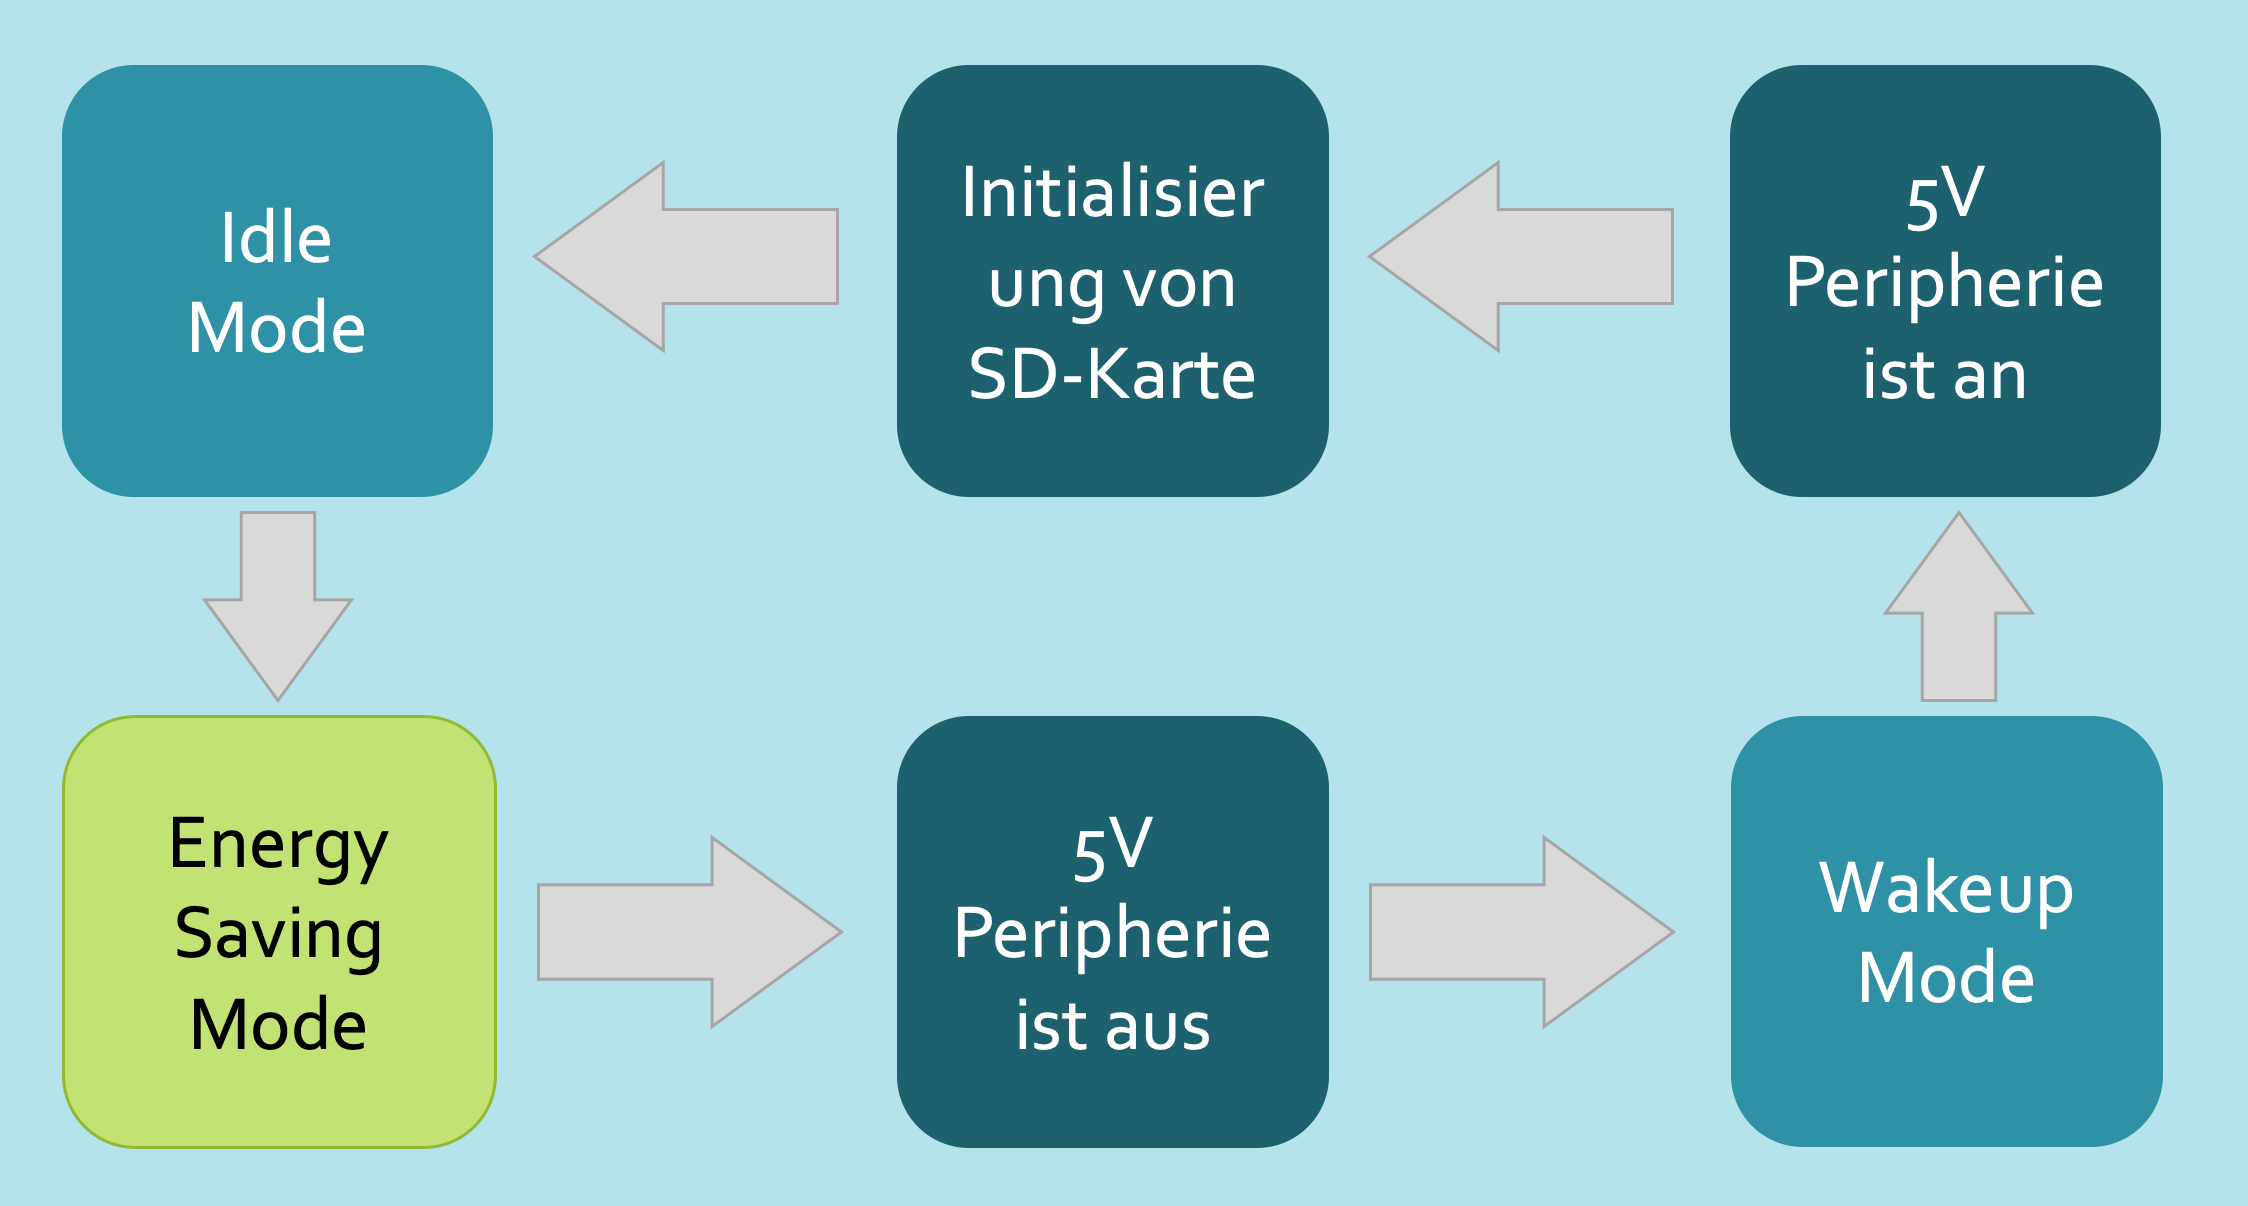
\includegraphics[width=12cm] {Idle State and Evergy Saving.png}
	\caption{Energy Saving Mode in Idle State}
    \label{fig. energysavingmode}
\end{figure}

\subsubsection{Akku-, BT-, SD-Abfrage}

Ausßerhalb der switch-Anweisung, die die \textit{State Machine} bildet, werden jede Sekunde folgende Funktionen aufgerufen:
\begin{itemize}
    \item \textit{ADC\_Akku\_Average\_Value} berechnet über drei Sekunden den Mittelwert der ADC-Werte der Akkuspannung. Dieser wird als Prozentangabe an das Display gesendet.
    \item \textit{Check\_BT\_Connection} und \textit{Check\_SD\_Card\_Connection} sind zwei Funktionen, welche die aktuelle Verbindung der Peripherie zum Bluetooth-Modul sowie zum SD-Kartenleser ermitteln und auf dem Display anzeigen. Hierfür werden die \textit{State-Pins} der Module abgefragt. Besteht eine Verbindung zum jeweiligen Modul, sind die Symbole auf dem Display blau, anderenfalls sind diese grau. Der Start einer Langzeitaufnahme ist nur mit angeschlossener SD-Karte möglich.\\
    Bei der Abfrage für die SD-Karte gibt es außerdem zwei zusätzliche Funktionen. Wenn die SD-Karte herausgezogen wird, erscheint auf dem Display eine Warnmeldung. Beim Entfernen und wieder Anschließen einer SD-Karte, wird diese neu initialisiert und die aktuellen Daten bleiben vorhanden.
\end{itemize}

\input{ekg_7_realisierung_gehäuse}

%!TEX root =  ..\ekg_7_projektbericht.tex

%EKG-7 Realisierung/Schnittstellen

\subsection{Schnittstellen}


%TODO Verweis auf Kapitel UART zu Bildschirm einfügen
\subsubsection{Schnittstelle zum Bluetooth Modul + DMA}

Das verwendete Bluetooth Modul HC-05 wird über UART angesprochen. Die Baudrate ist dabei flexibel konfigurierbar. Das Modul öffnet auf dem verbundenem Smartphone oder Laptop einen virtuellen COM-Port, an welchen es alle ihm übertragenen Daten weiterleitet. Seitens der MCU wird das Hardware-Modul USCI\_A1 verwendet, welches mit Ausnahme der Basisadresse identisch zu USCI\_A0 in Kapitel ??? initialisiert wird. \\

Um beim versenden der Nachrichten keine Verzögerung oder zusätzliche CPU Last zu verursachen, wird Direct Memory Acces (DMA) verwendet. Das DMA-Modul kann nach korrekter Initialisierung automatische Daten im Hintergrund in das TX Register des UART Moduls kopieren. Hierfür muss im DMA Modul der Transfermodus Single Transfer eingestellt werden. Weitere benötigte Konfigurationen sind Byte-to-Byte Transfer, die Quelladresse, die Zieladresse und die Datengröße. Als Trigger um das nächste Byte zu übertragen ist das Interrupt Flag UCA1TXIFG zu wählen, welches immer dann aktiv ist, wenn das UART Modul bereit ist ein weiteres Byte zu senden. Damit ein ganzer String gesendet werden kann, ist das DMA Modul auf ein Inkrementieren der Quelladresse nach jedem versendetem Byte einzustellen. Somit wird nach Aktivierung des Moduls durch setzen des DMAEN Bits ein kompletter String im Hintergrund Byte für Byte versendet, bis die vorgegebene Datengröße abgearbeitet ist und das DMAEN Bit automatisch zurückgesetzt wird. Die CPU selbst wird dabei jeweils nur für zwei Takte durch das DMA Modul unterbrochen und muss nicht auf den Abschluss jedes Sendevorgangs warten.

%EKG-7 Android-App
\subsection{Android-App}
Dieses Unterkapitel behandelt den Entwurf und die Entwicklung der Home-EKG Android App zur Darstellung eines EKG Signals unter Verwendung der Bluetooth 2.0 Technologie. Die Kommunikation mit einer Datenbank ermöglicht es in Echtzeit Patientendaten zu speichern, sowie Authentifizierungsabfragen durchzuführen. Das Projekt wurde hauptsächlich mit der objektorientierten Programmiersprache Java realisiert. 

\subsubsection{Datenbank}
Um eine geräteübergreifende Funktionalität aller Features der Android App zu gewährleisten wurde bei der Entwicklung auf die Echtzeitdatenbank \textit{Firebase} \cite{Firebase}  zurückgegriffen. Die von Google bereitgestellte IDE Android Studio \cite{Android_Studio} ermöglicht eine besonders einfache Implementierung der verschiedenen Funktionalitäten der Datenbank wie Authentifizierung und Cloud-Speicherung. \\
Bei der Registrierung eines Anwenders wird ein neuer \textit{Child-Node} im Benutzer-Baum angelegt und mit einer individuellen Identifikationsnummer ausgestattet. Über diese kann die App mit dem Server kommunizieren und Daten austauschen. \\
Der Benutzer hat außerdem die Möglichkeit ein Profilbild im .png Format hochzuladen, welches in einen von \textit{Firebase} verwalteten externen Speicher abgelegt wird. Durch die Verwendung von Google Analytics \cite{Google_Analytics} kann ferner das Nutzerverhalten statistisch erfasst und auf verschiedene Arten ausgewertet werden. 

\subsubsection{Aktivitäten}

\begin{wrapfigure}[12]{R}{0.4\textwidth}
\vspace{-25pt}
\includegraphics[width=0.4\textwidth]{app_Activity.png}
\caption{Lebenszyklus}
\label{app_Activity}
\end{wrapfigure}

Jede \textit{Activity}-Klasse \cite{Activity_Overview} stellt einen Bildschirm (Login Seite, Register Seite oder Profil Seite) der App dar, mit welcher der Benutzer interagieren und somit Befehle an das Betriebssystem weitergeben kann. Beim Start einer neuen Aktivität wird eine Instanz der zugrunde liegenden Java Klasse erzeugt und der zugehörige Lebenszyklus (Abbildung \ref{app_Activity} \cite{Activity_Lifecycle}) gestartet.
Um zwischen den drei Hauptzuständen

\begin{itemize}
\item[•] Aktivität läuft im Vordergrund und hat Fokus
\item[•] Aktivität läuft im Hintergrund
\item[•] Aktivität wurde gestoppt
\end{itemize}

zu wechseln, bietet die \textit{Activity} Klasse außerdem einen Satz von sechs \textit{Callback} an, die bei Übergängen von verschiedenen Phasen des Lebenszyklus aufgerufen werden. Durch Verwendung der \textit{onCreate()} Methode können so zum Beispiel Buttons oder Textfelder initialisiert werden.
Die Home-EKG App besteht insgesamt aus sieben Aktivitäten, welche im Folgenden einzeln vorgestellt werden.

\begin{itemize}
\item Login und Registrierung Aktivität: Die Login Aktivität (Abbildung \ref{app_login_reg} links) stellt den Einstieg des Benutzers in die App dar. Grundlegend werden drei Login Varianten angeboten, wobei der Benutzer nur bei der Methode über E-Mail einen neuen Account anlegen muss, bevor er die App verwenden kann. Die Implementierung der Services von Facebook und Google erlauben es dem Nutzer sich über bereits bestehende Accounts anzumelden, ohne eine erneute Registrierung vornehmen zu müssen. \\
Außerdem besteht die Möglichkeit durch Setzten des Hakens im Feld \textit{Remember me} die Daten für zukünftige Anmeldeversuche lokal in einem privaten \textit{SharedPreferences}-Objekt zu speichern, um beim nächsten Start der App die Login Seite zu überspringen und direkt zur Main Aktivität weitergeleitet zu werden. \\
Bei Betätigung des Login Buttons wird eine Verbindung zum Server der Datenbank aufgebaut und die in den zwei TextInput-Feldern eingegebenen Zeichen an Googles \textit{Firebase} geschickt. Bei erfolgreichem Abgleich werden die Benutzerdaten vom Server heruntergeladen und der Benutzer zum Main Screen weitergeleitet. \\
Durch einen Klick auf \textit{Register Now} oder Plus wird eine neue Registrierungs-Aktivität gestartet (Abbildung \ref{app_login_reg} rechts). Die Felder Name, Passwort und E-Mail sind verpflichtend auszufüllen. Durch Versenden einer Bestätigungs-Mail wird die Validität der Adresse überprüft und der Account erst nach erfolgreicher Bestätigung erstellt.
	\begin{figure} [!h]
		\begin{center}
			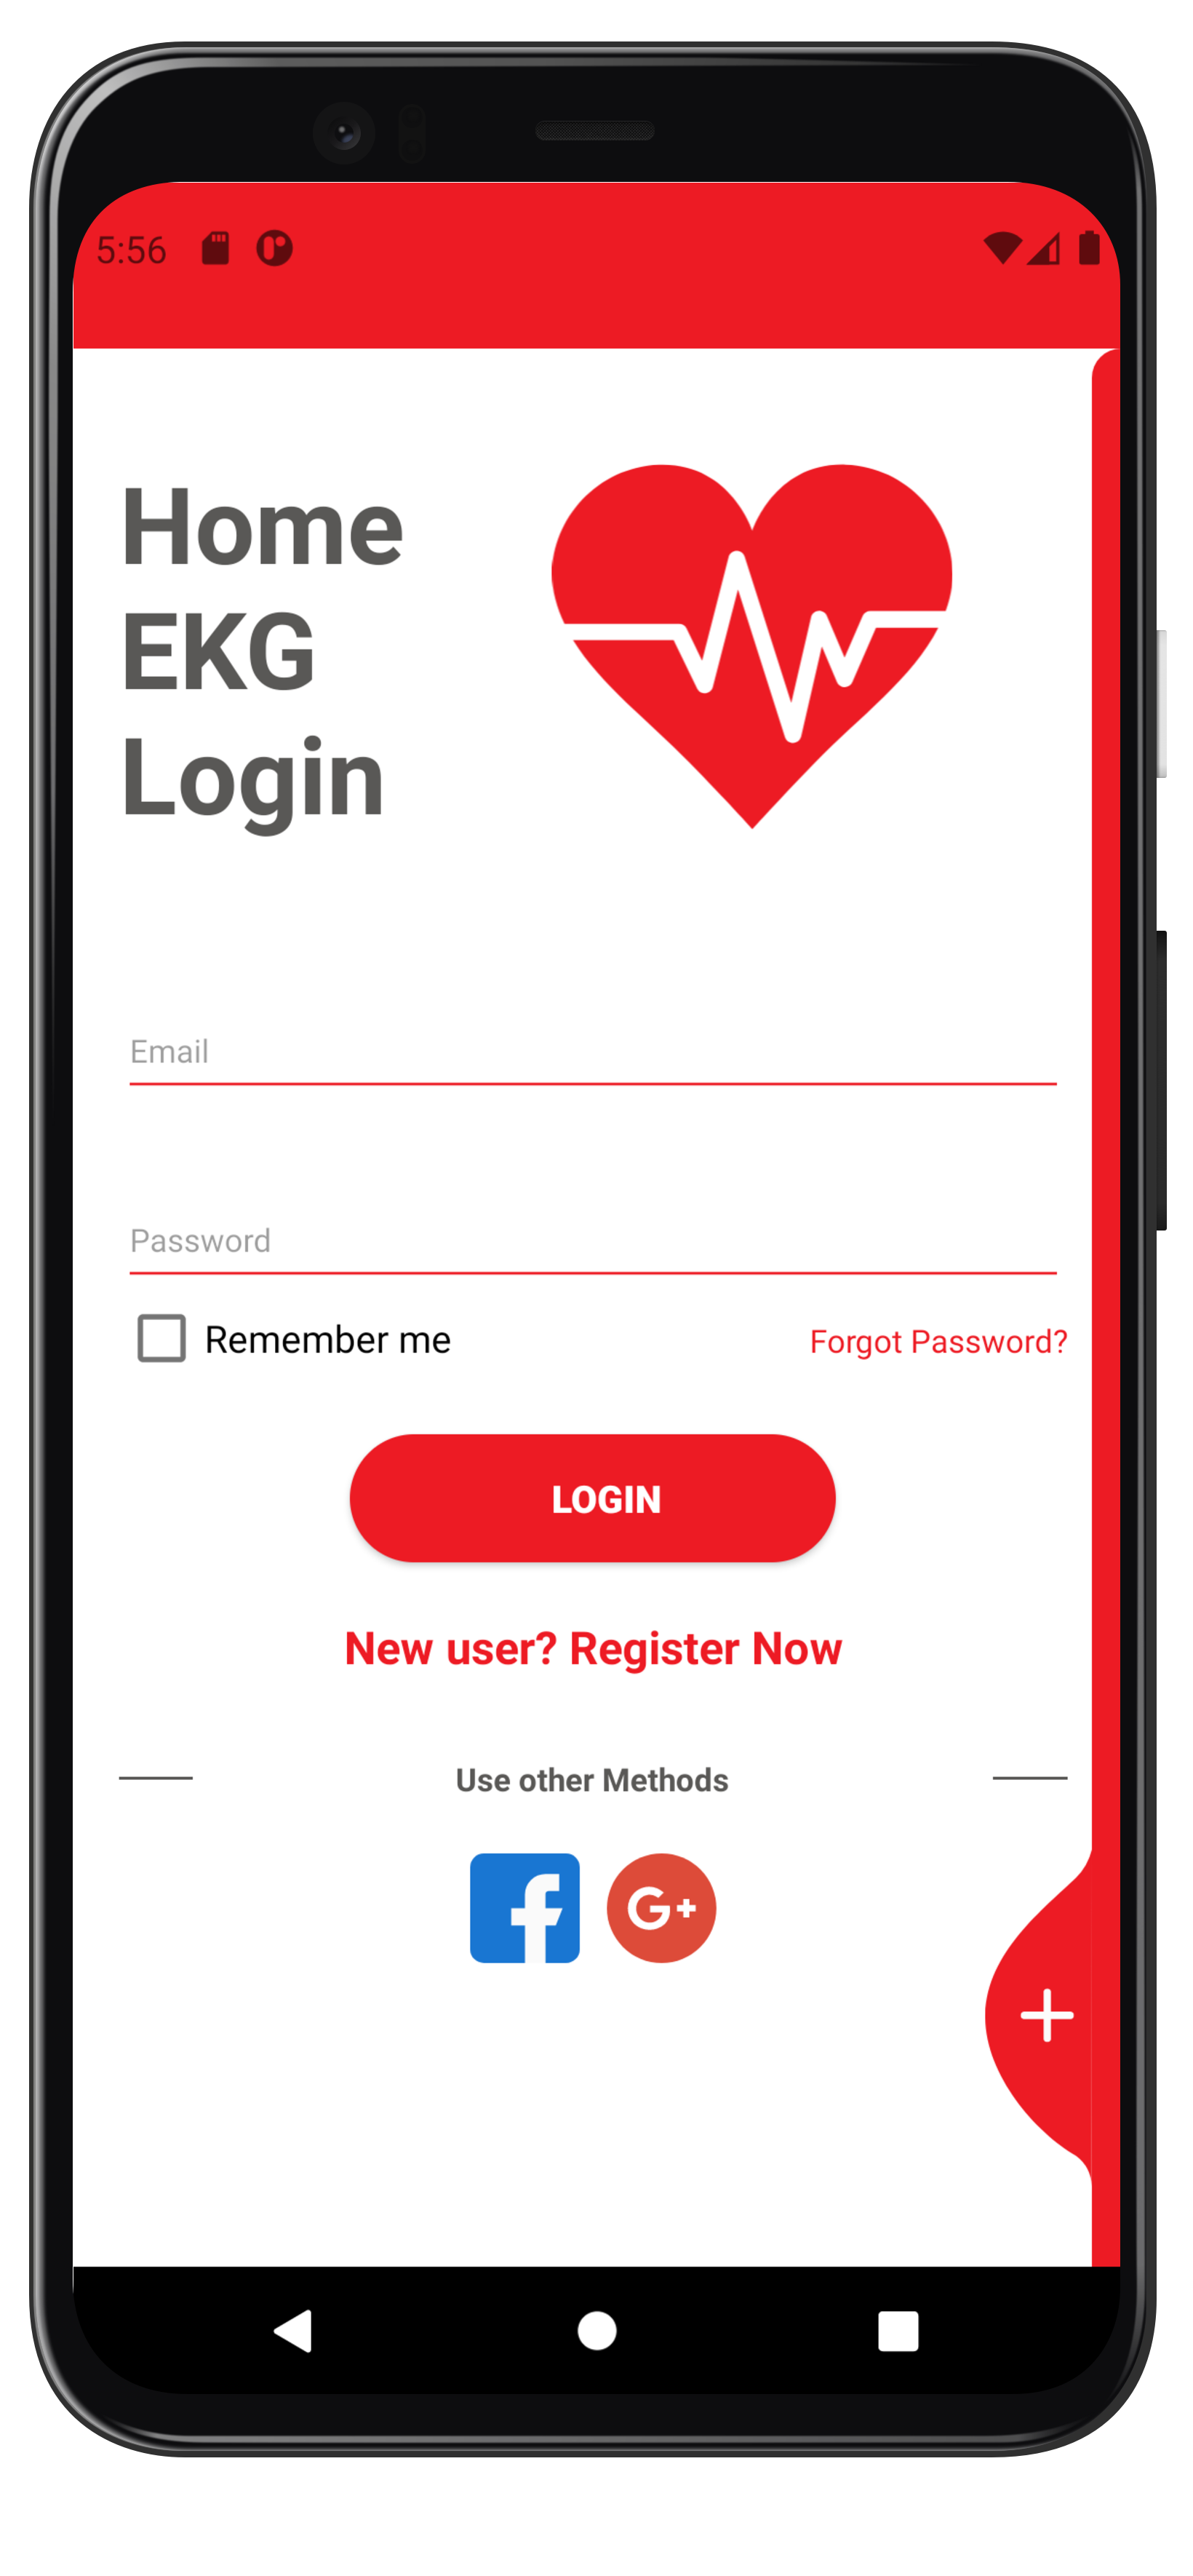
\includegraphics[width=150pt]{app_login.png}
			\hspace{1.5 cm}
			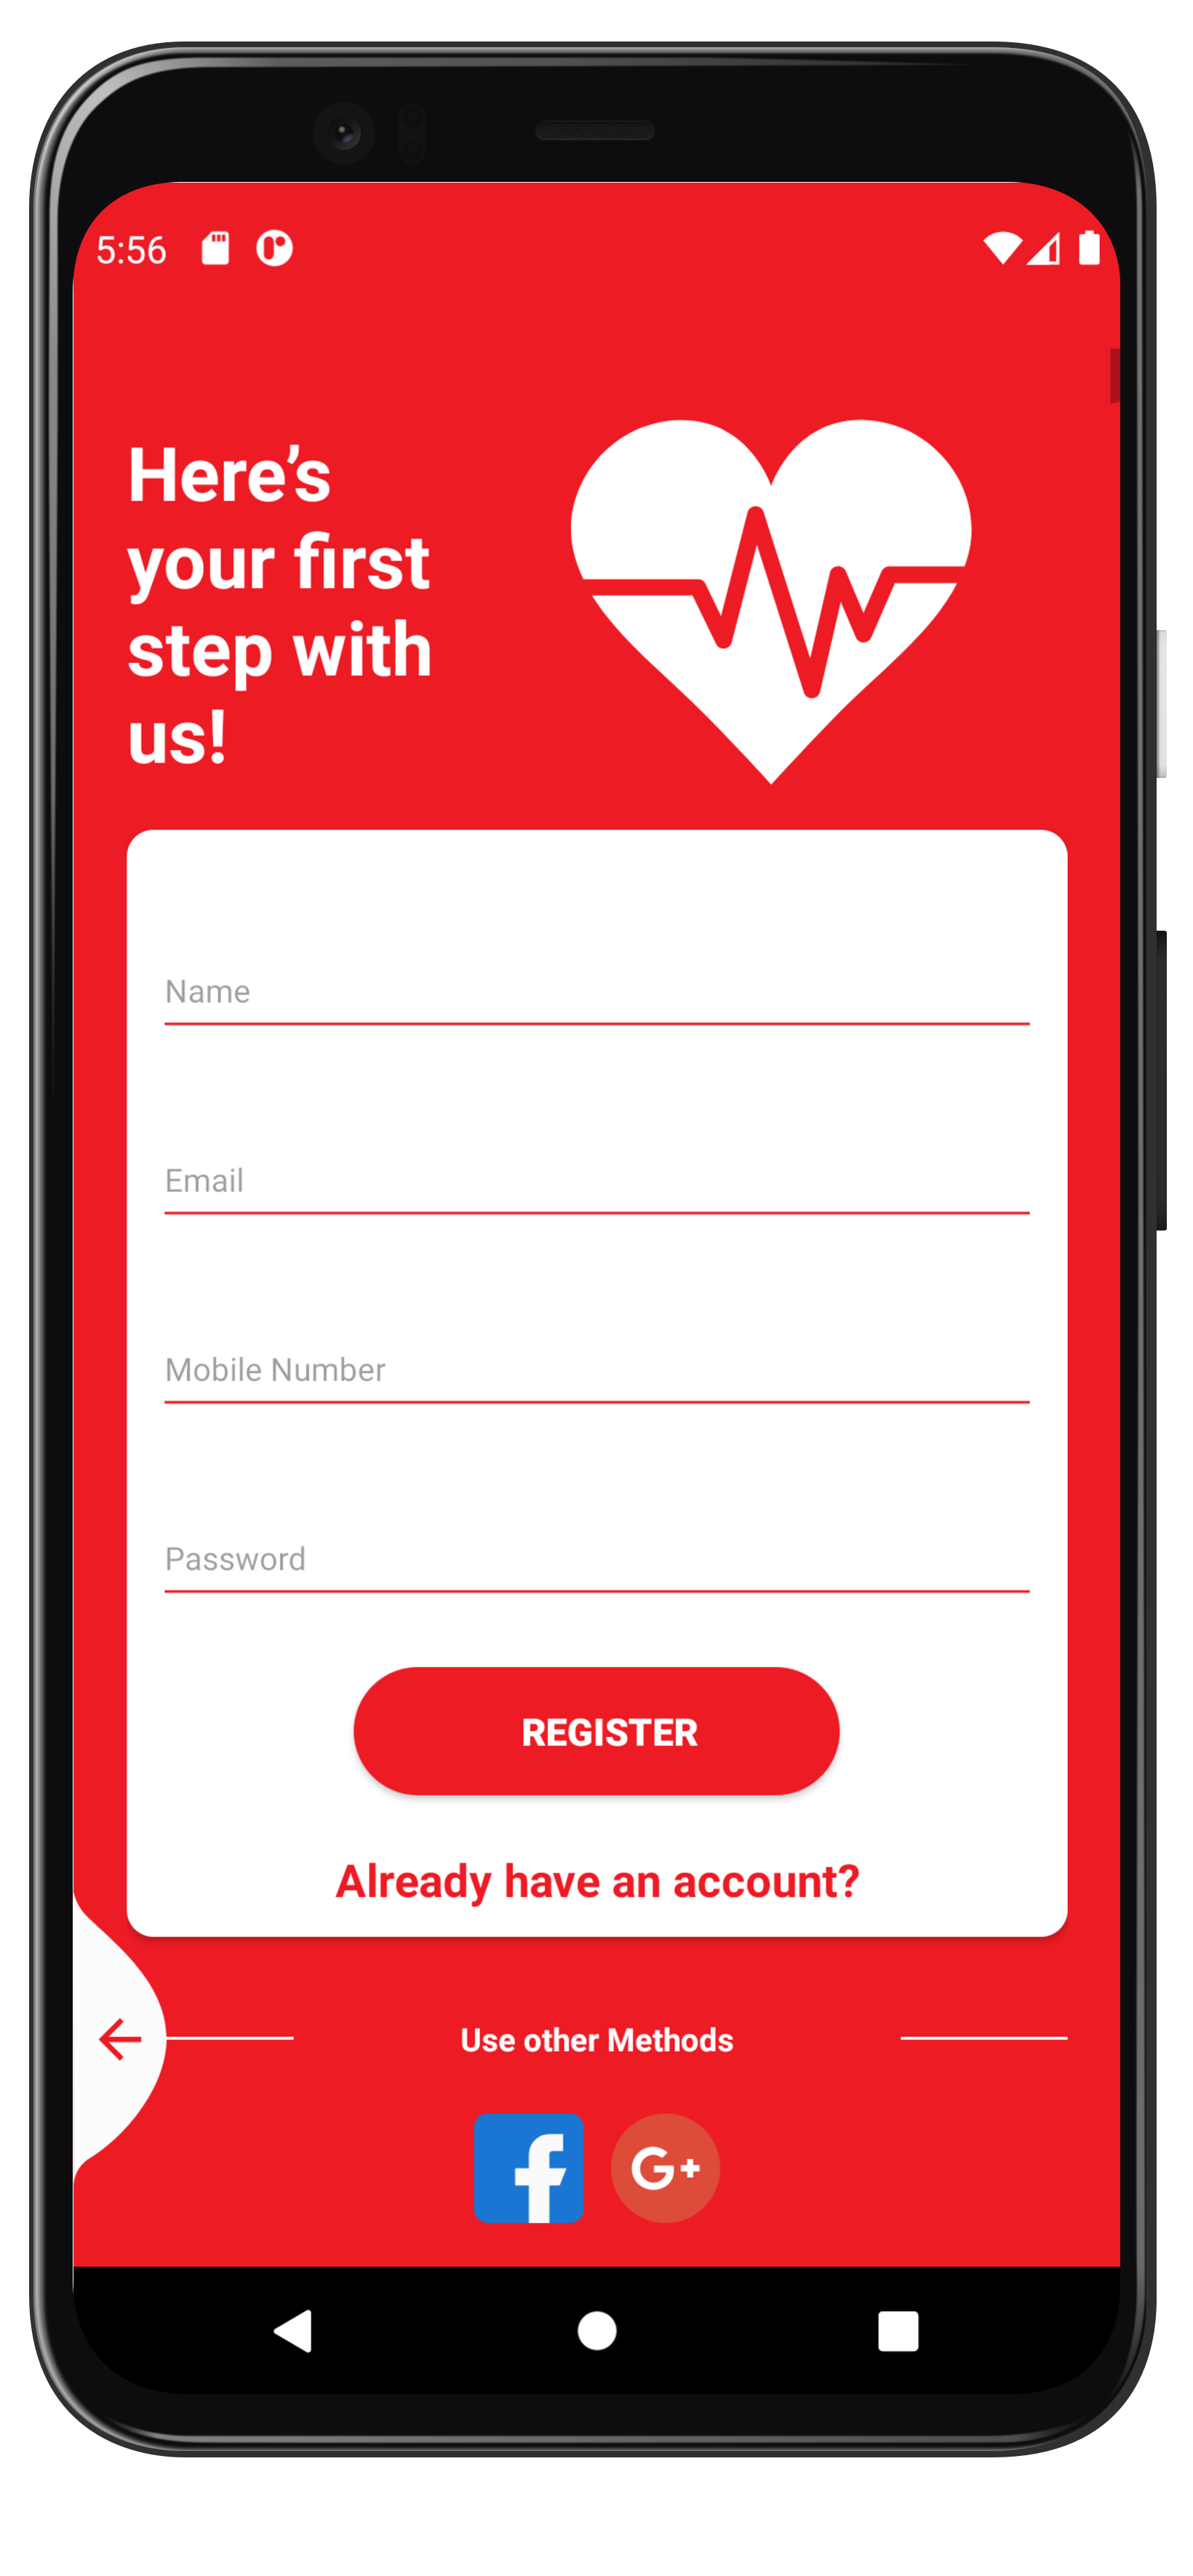
\includegraphics[width=150pt]{app_register.png}
		\end{center}
		\caption{Login und Registrierungs Aktivität}
		\label{app_login_reg}
	\end{figure}

\item Home Aktivität: Die Home Aktivität (Abbildung \ref{app_profile_scan} links) stellt dem Benutzer eine Schnittstelle zum Datenbank Server bereit, um seine Daten erstmalig hochzuladen und zu einem späterem Zeitpunkt aktualisieren zu können. Wird zum Beispiel das Gewicht verändert und eine Update Anfrage an \textit{Firebase} geschickt, wird auch nur dieser \textit{Child Node} der Benutzerreferenz aktualisiert und nicht das ganze Profil erneut hochgeladen. \\
Durch einen implementierten \textit{onDataChange()} Listener werden serverseitige Änderungen auch direkt in Echtzeit auf der Home Aktivität aktualisiert, ohne dabei eine ständige Verbindung halten zu müssen. Die folgenden Attribute sind personalisierbar: Mail, Geschlecht, Geburtsdatum, Größe, Gewicht, Wohnort und Versicherung.\\
Durch Drücken auf das Stift-Symbol unterhalb des Profilbildes, wird ein \textit{Action Intent} generiert, der die auf dem Smartphone als standardmäßige eingestellte Galerie öffnet und den Benutzer ein personalisiertes Profilbild auswählen lässt. Im \textit{onActivityResult()} Callback wird dem Foto eine URI zugeordnet und in den \textit{Firebase}-Speicher hochgeladen. Bei einem Login über ein anderes Gerät wird nun auch das neue Profilbild angezeigt und lokal im Speicher hinterlegt, um den Internetdatenverbrauch zu minimieren. \\
Über das Dropdown Menu in der oberen rechten Ecke kann der Benutzer einen Abmeldedialog starten, wobei auch die \textit{Shared Preferences}-Variable der Auto Login Checkbox zurückgesetzt wird. Der Button „Connect to EKG“ leitet den Benutzer zur Signal Aktivität weiter.
\begin{figure} [!h]
	\begin{center}
		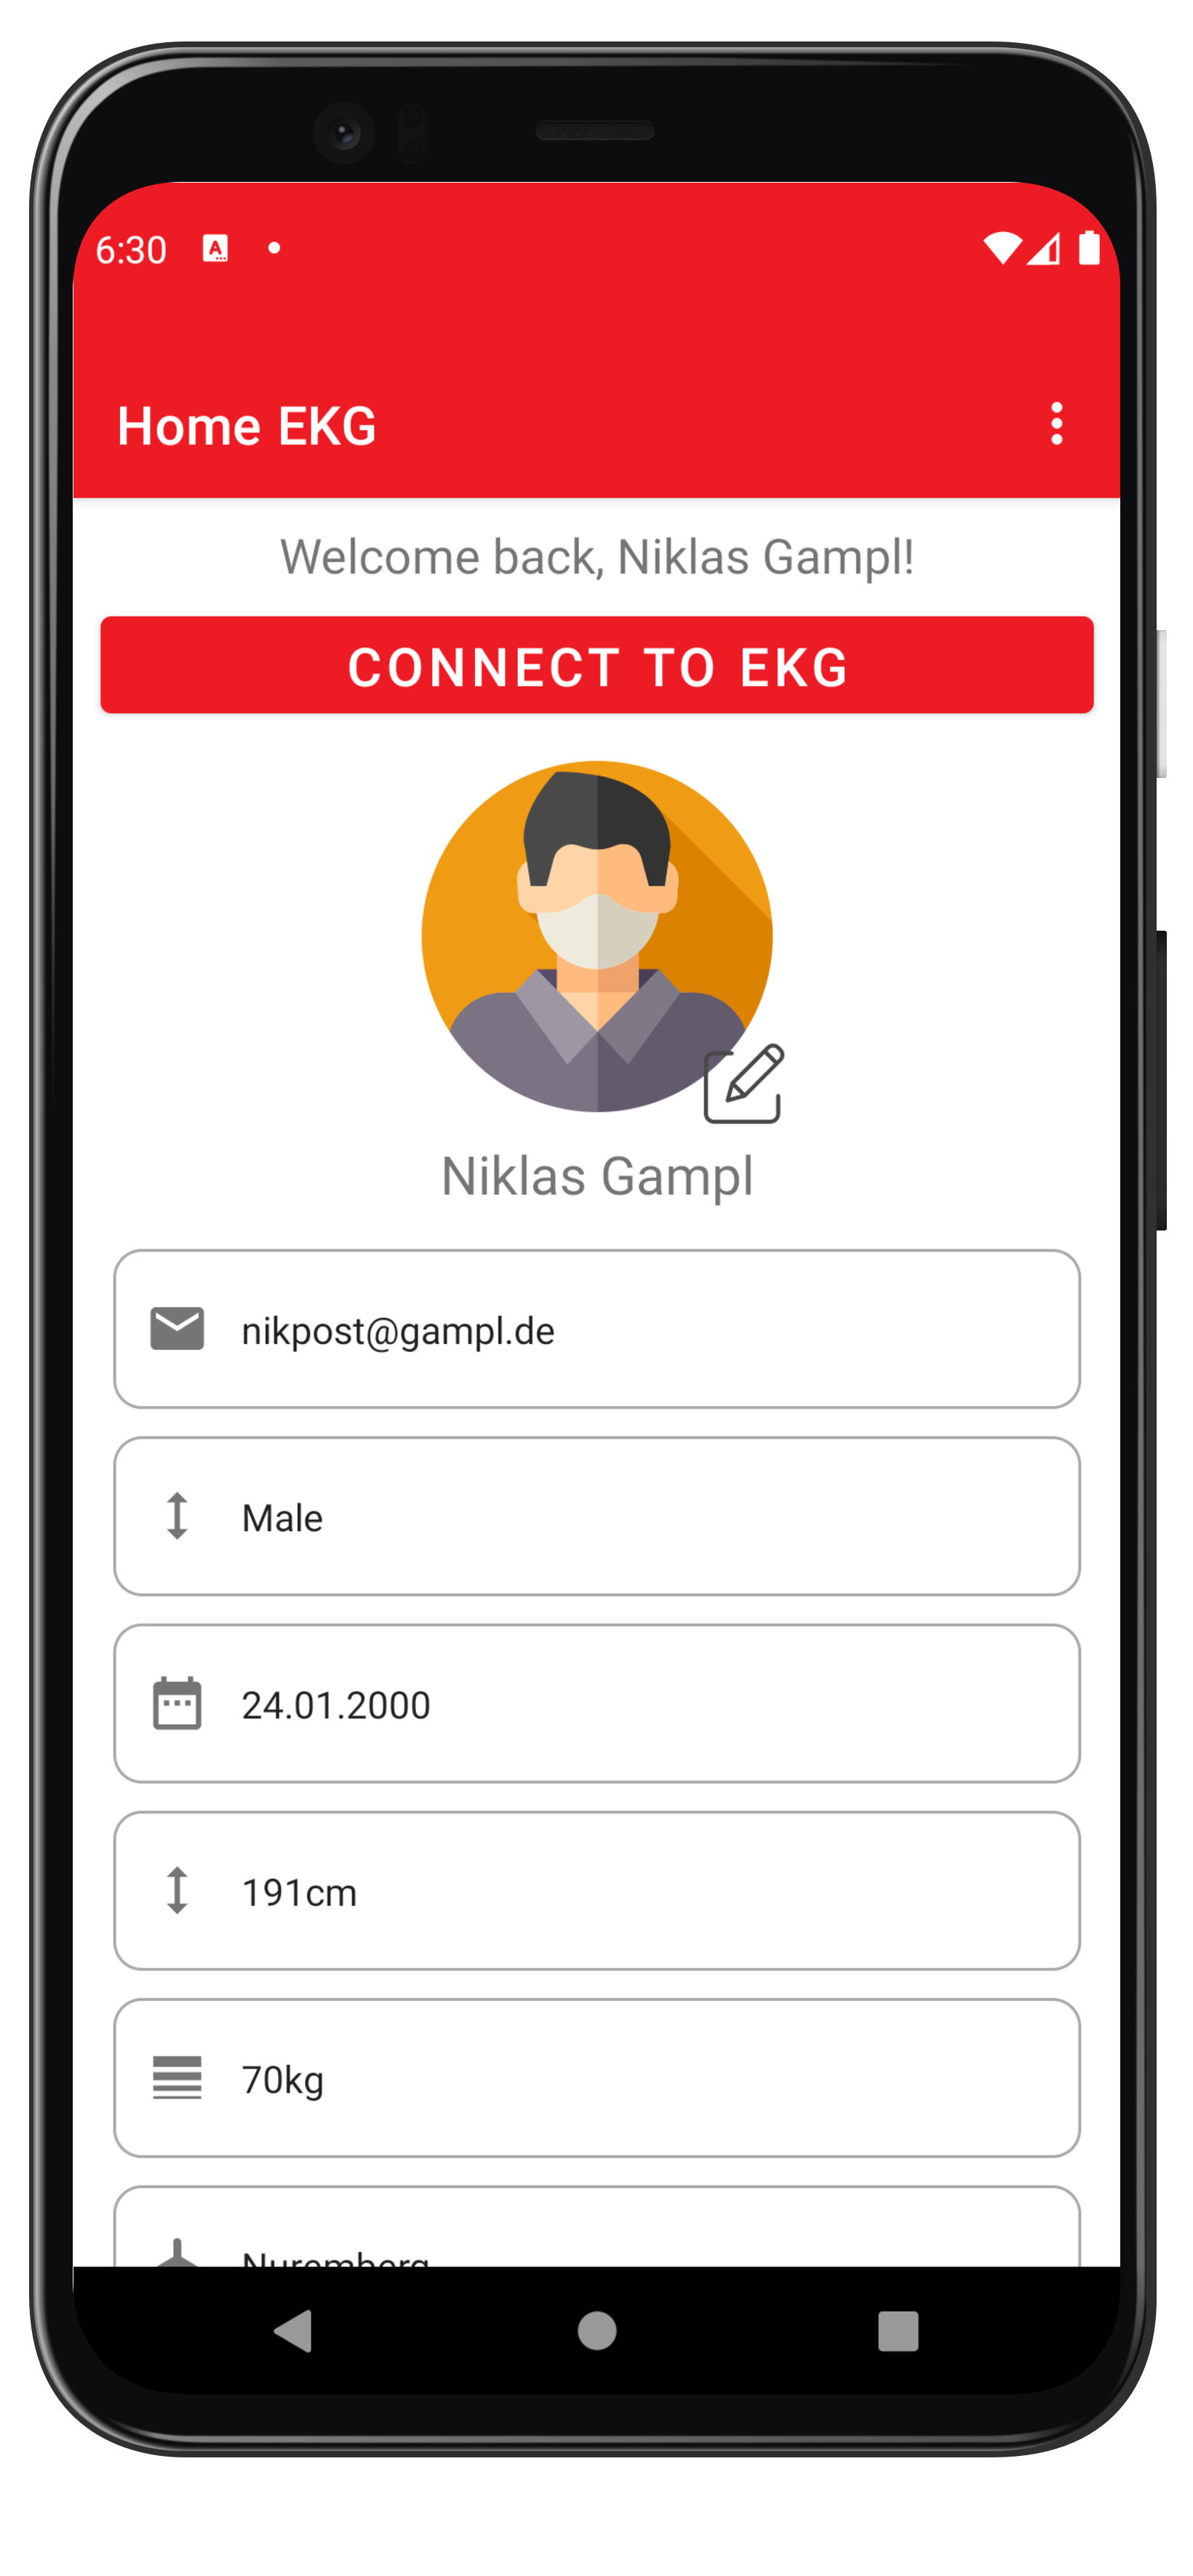
\includegraphics[width=150pt] {app_profile.png}
		\hspace{1.5 cm}
		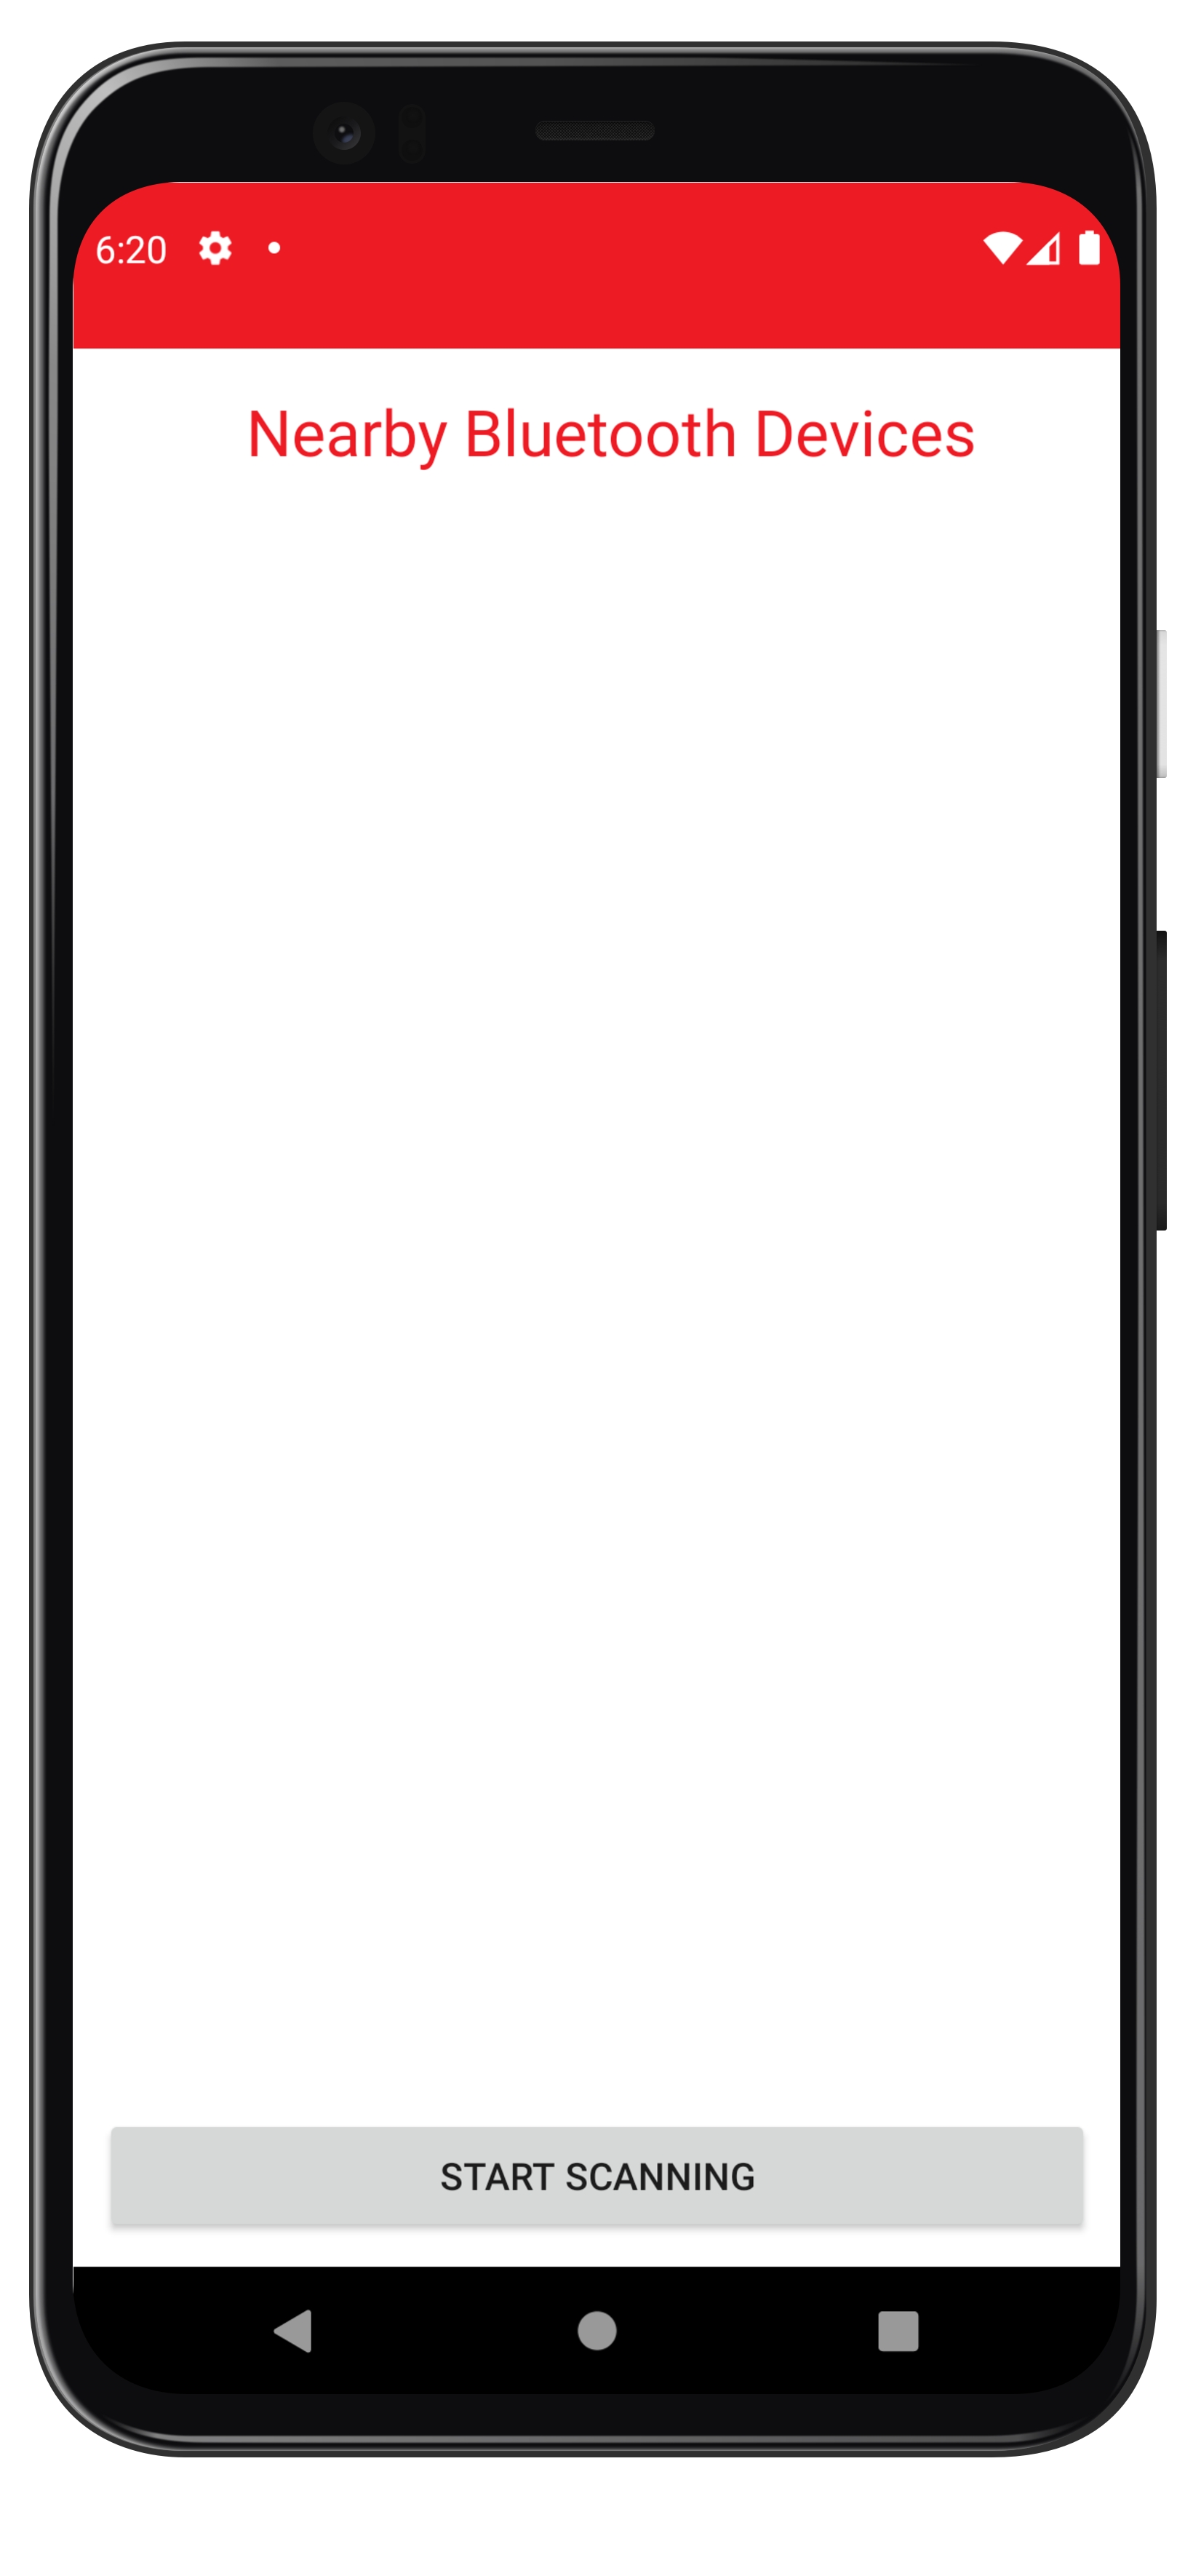
\includegraphics[width=150pt] {app_scan.png}
	\end{center}
	\caption{Profil und Scanner Aktivität}
	\label{app_profile_scan}
\end{figure}

\item Signal und Scanner Aktivität: Die Signal Aktivität (Abbildung \ref{app_signal}) stellt die Hauptfunktionalität der App, das Anzeigen eines Echtzeit EKG Signals, bereit. Durch Drücken auf den Connect Button wird der Benutzer zur Scanner Aktivität (Abbildung \ref{app_profile_scan} rechts) weitergeleitet und aufgefordert Bluetooth zu aktivieren, falls dies nicht bereits geschehen ist. \\
Um nach Bluetooth Geräten in der Umgebung scannen zu dürfen, muss der Benutzer der App erst die Berechtigung zur Standortfreigabe erteilen, da andere Geräte dadurch auf den Ort des Geräts schließen können.\\
Ein Klick auf Start Scanning ruft unter anderem die \textit{startDiscovery()} Methode des BluetoothAdapter Objekts auf. Sobald ein Gerät gefunden wurde, wird es mit Namen und zugehöriger Mac-Adresse in ein ListView Layout eingefügt und im internen Gerätespeicher ein Abgleich gestartet, ob dieses Gerät bereits gepaired ist. \\
Durch Auswahl des EKG7-Geräts versucht die Home EKG App eine Verbindung herzustellen und gibt bei Erfolg eine Toast Nachricht aus. Die App wird die Verbindung nun solange aufrecht erhalten, bis diese vom System durch Inaktivität geschlossen wird oder der Disconnect Button in der Signal Aktivität gedrückt wird. In einem neuen Thread wird der InputStream der etablierten Verbindung kontinuierlich in einen Buffer geschrieben und die Daten durch einen Handler an die Signal Aktivität weitergeleitet. Die OpenSource Grafik-Bibliothek GraphView \cite{Graph_View_Libary} ist für das Zeichnen des Signals zuständig.
\begin{figure} [!h]
	\begin{center}
		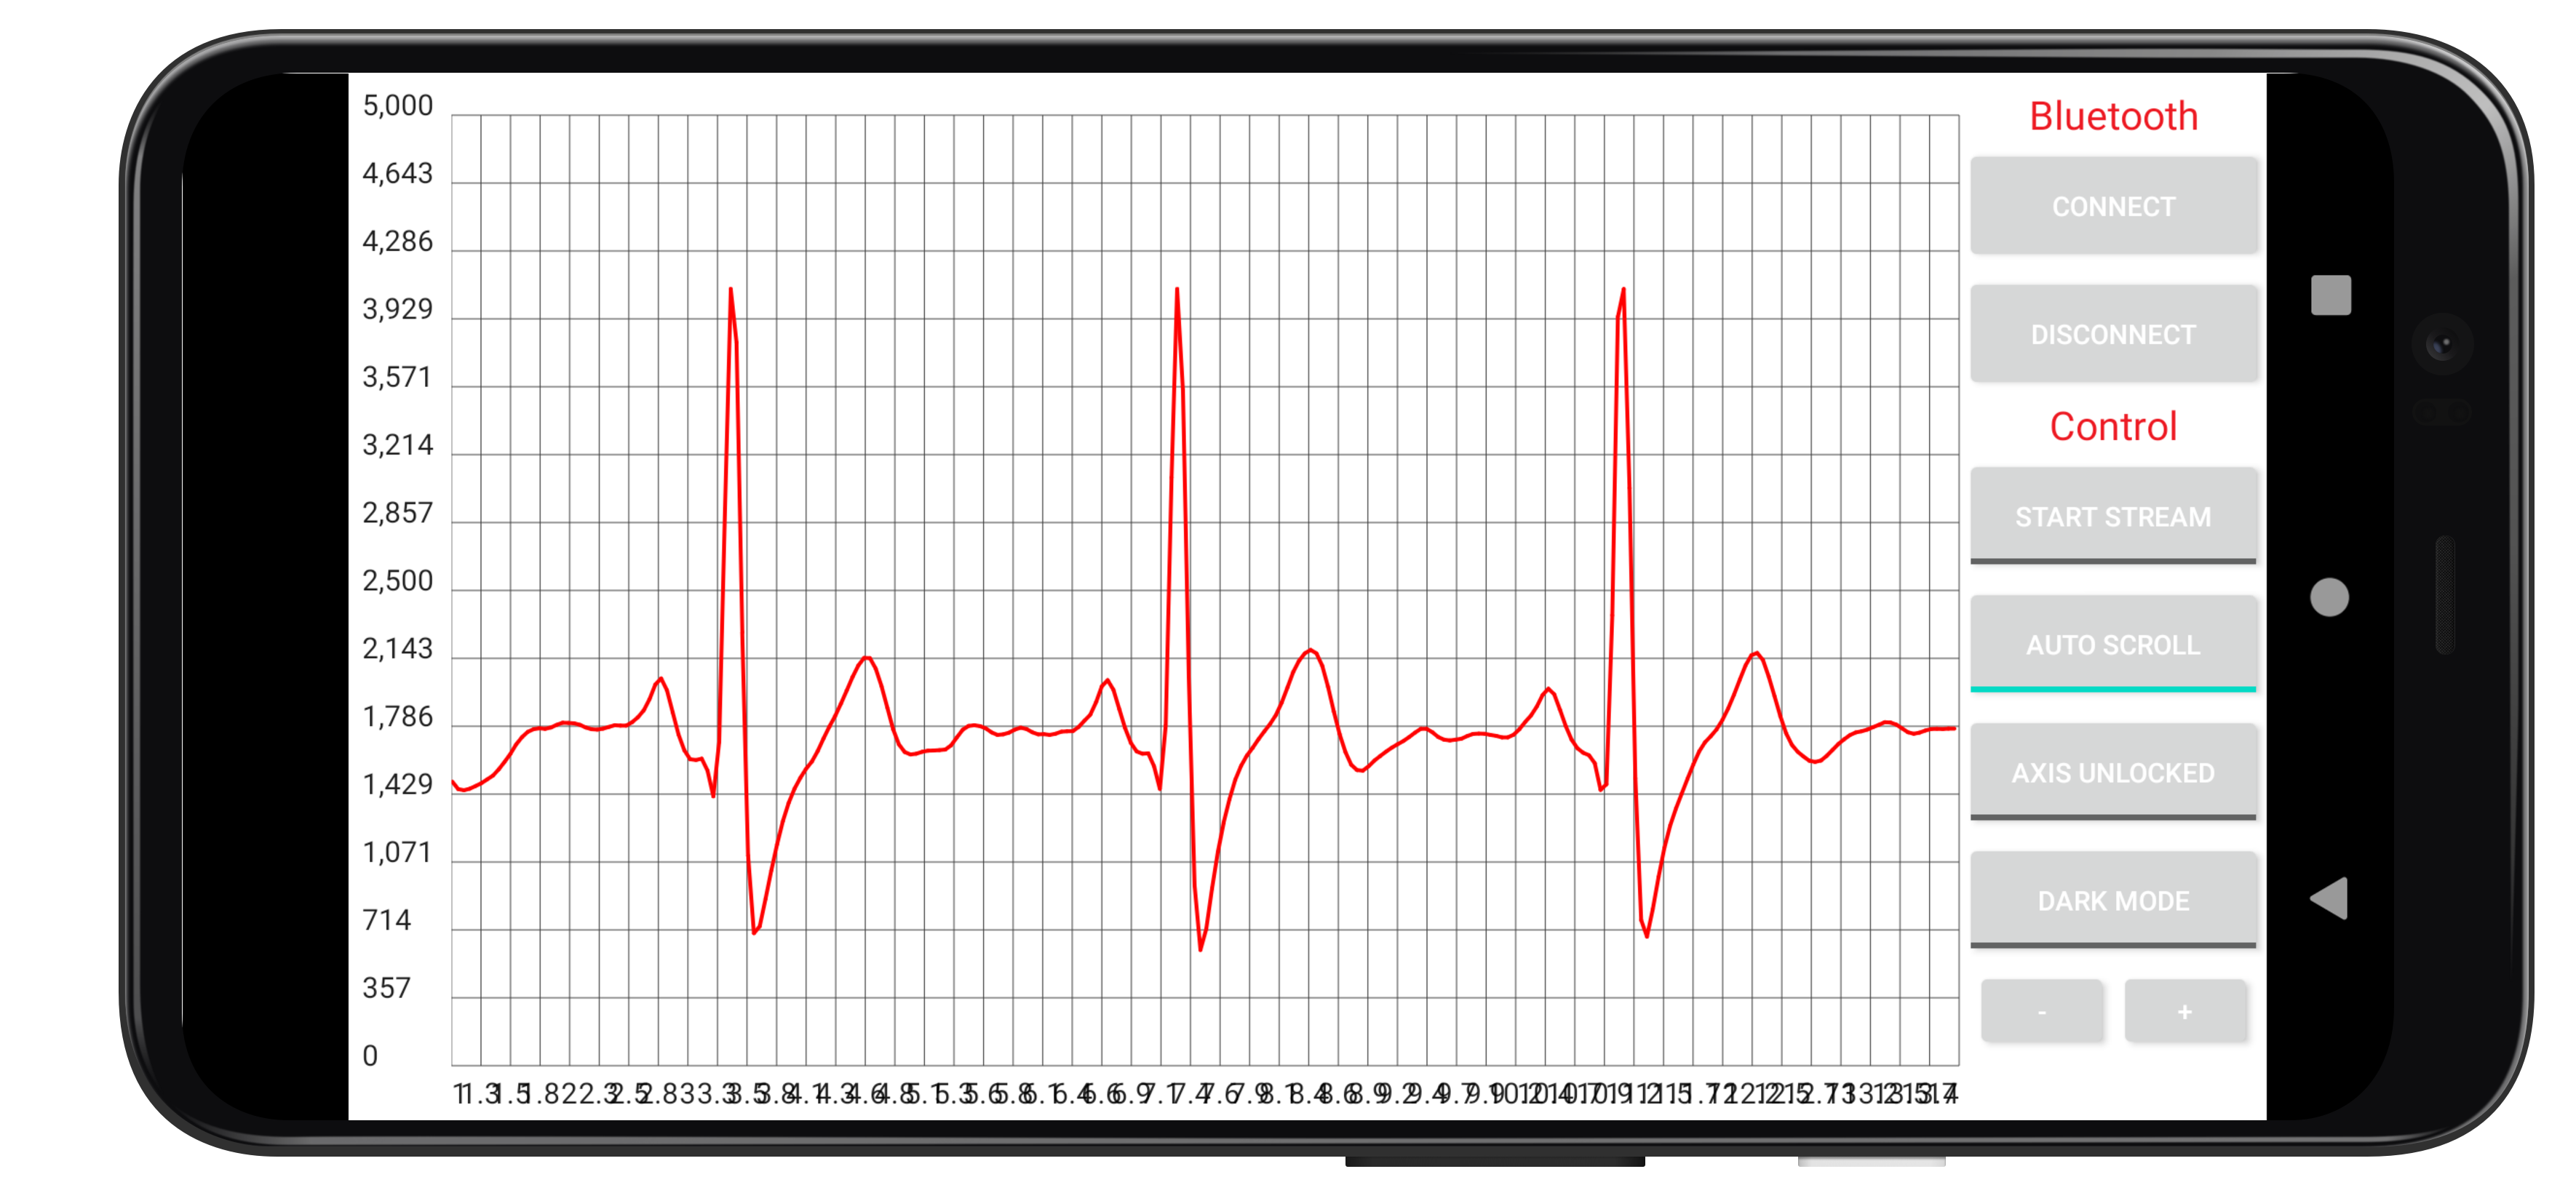
\includegraphics[width=\textwidth] {app_signal.png}
	\end{center}
	\caption{Signal Aktivität}
	\label{app_signal}
\end{figure}
\end{itemize}

%EKG-7 Realisierung/SD-Karten-Speicher

\subsection{SD-Karten-Speicher}

%ekg_7_Realisierung/analoge_Filterschaltung

\subsection{Analoge Filterschaltung}

Dieses Unterkapitel befasst sich mit den einzelnen Stufen der analogen Filterschaltung und wie die Anforderungen an sie umgesetzt werden.

\subsubsection{Eingangsstufe}

Direkt an die Klebeelektroden sind die beiden symmetrischen Eingangskanäle angeschlossen. Sie sind hochohmig um die Signalquelle nicht zu belasten. Die Kanäle bestehen jeweils aus:

\begin{enumerate}

\item einem passiven Hochpass (fg = \SI{0,48}{\hertz}) zur Abtrennung des Gleichanteils und zur Kleinsignaleinkopplung auf das Gleichspannungspotential der Filterschaltung

\item einem passiven Tiefpass (fg = \SI{159}{\hertz}) zur Unterdrückung von hochfrequenten Störungen (>\SI{100}{\kilo\hertz}) bereits vor dem Differenzverstärker

\item einer bidirektionalen TVS-Dioden zum Schutz der Schaltung vor einem ESD

\end{enumerate}

\subsubsection{Differenzverstärkung}

Zur Differenzbildung der beiden Kanäle wird ein Instrumentenverstärker von Analog Devices (AD) verwendet. Das Modell AD8422ARMZ ist ein Rail-to-Rail-Verstärker der im niedrigen Frequenzbereich bis \SI{60}{\hertz} eine Gleichtaktunterdrückung von etwa \SI{120}{\decibel} erreicht. Dies unterdrückt Störsignale die durch externe elektromagnetische Felder in die Messleitungen eingekoppelt werden. Seine Verstärkung wird mittels eines \SI{33}{\ohm}-Widerstandes auf den Faktor 420 eingestellt, was etwa in \SI{52}{\decibel} entspricht. Diese Vorverstärkung sorgt dafür, dass das Signal auf dem Weg durch die Filterschaltung robuster gegen Störungen ist. Da das EKG-Gerät über einen Akku betrieben wird, muss der Instrumentenverstärker mit einer unipolaren Versorgungsspannung arbeiten. Sein Versorgungsstrom von etwa \SI{330}{\micro\ampere} ist ebenfalls gut für einen Akkubetrieb geeignet. %TODO Quelle Datenblatt AD8422ARMZ

\subsubsection{Kerbfilter}

Da der Körper eines Menschen aus leitendem Material besteht, können elektromagnetische Störfelder eine Spannung in ihm induzieren. Diese Wechselspannung mit einer Amplitude von bis zu \SI{100}{\milli\volt} und einer Frequenz von \SI{50}{\hertz} überlagert das EKG-Signal des Herzens. Um diese Netzschwingung zu unterdrücken, wird ein Doppel-T-Filter verwendet. Bei idealen Bauteilen erreicht diese aktive Bandsperre eine Güte von annähernd 0,5 und eine Dämpfung von \SI{76}{\decibel}. Da jedoch die verwendeten SMD-Widerstände und Kondensatoren nur mit unvermeidbaren Toleranzen erhältlich sind, fällt die effektive Dämpfung auf \SI{20}{\decibel} bis \SI{30}{\decibel}. Dies wäre für die Anwendung nicht ausreichend, daher werden in der Schaltung zwei dieser Bandsperren in Reihe geschaltet. Die im Schaltplan vorgesehenen Parallelschaltungen der Widerstände dienen dazu die Widerstandswerte flexibel einzustellen, um auch noch im Nachhinein auf die Toleranzen der Kondensatoren reagieren zu können. %TODO Verweis auf Anhang Schematic analoge Filterschaltung

\subsubsection{Tiefpassfilterung}

Bei den benötigten Operationsverstärkern wurde ein Vierfach-OPV von Analog Devices gewählt. Zwei der Operationsverstärker werden für die \SI{50}{\hertz}-Filter verwendet, die anderen zwei dienen der Tiefpassfilterung und Nachverstärkung. Der AD8544ARZ ist ein Rail-to-Rail-Verstärker der mit einem geringen Versorgungsstrom von \SI{45}{\micro\ampere} auch unipolar betrieben werden kann. Da das zu filternde Signal im niederfrequenten Bereich liegt, ist er mit seinem Verstärkungs-Bandbreite-Produkt von \SI{1}{\mega\hertz} mehr als ausreichend. Mit dem Analog-Digital-Umsetzer (ADC) wurde eine Abtastfrequenz von \SI{1}{\kilo\hertz} angestrebt, die im Laufe der Entwicklung auf \SI{250}{\hertz} gesenkt wurde. Das Signal wird daher durch Tiefpässe begrenzt. Die Tiefpassfilterung setzt sich aus vier passiven Tiefpässen erster Ordnung und einem aktiven Tiefpass zweiter Ordnung zusammen. Die passiven Filter sind zwischen den aktiven Stufen der Schaltung eingebettet. %TODO Quelle Tietze-Schenk

\begin{figure} [!h]
	%\centering
	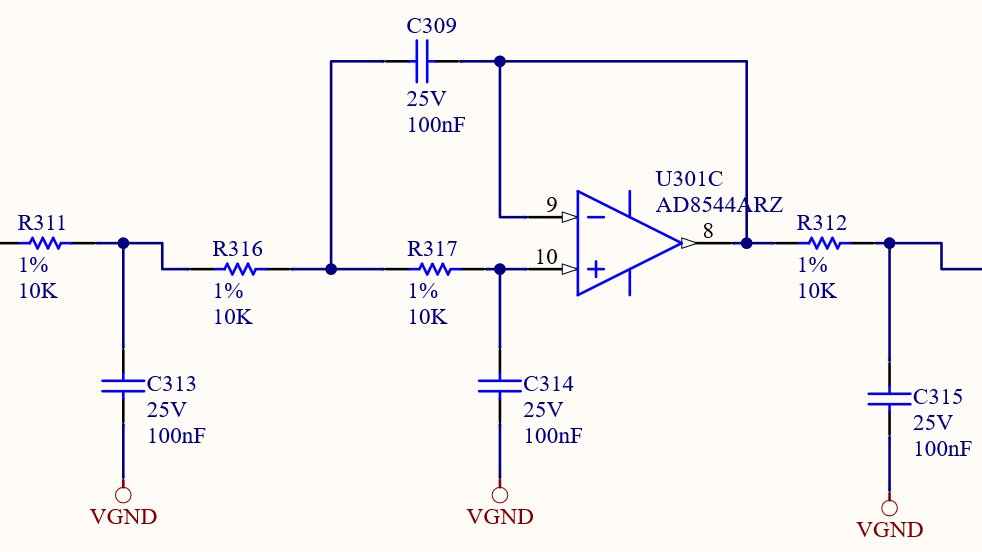
\includegraphics[width=\textwidth] {EKG_aktiver_Tiefpassfilter.png}
	\caption{Aktiver Tiefpass eingeschlossen von zwei passiven Tiefpässen}
	\label{aktiver Tiefpass} 
\end{figure}

In Abbildung \ref{aktiver Tiefpass} ist der verwendete aktive Tiefpass, realisiert durch eine Sallen-Key-Schaltung, abgebildet. Davor und danach befinden sich einfache passive Tiefpässe. Die zwei verbleibenden passiven Tiefpassfilter-Stufen befinden sich in der Eingangsstufe und zwischen den beiden \SI{50}{\hertz}-Filtern. Insgesamt ergibt sich damit eine Tiefpassfilterung sechster Ordnung, also eine Dämpfung von \SI{120}{\decibel} pro Dekade, über die Schaltung. %TODO Quelle Titze-Schenk

\subsubsection{Nachverstärkung}

Die Signalamplitude der Quelle beträgt nur etwa \SI{1}{\milli\volt}. Der ADC arbeitet in einem Bereich von \SI{0}{\volt} bis \SI{3}{\volt}. Um diesen Bereich bestmöglich zu nutzen muss das Signal auf eine Amplitude von etwa \SI{2}{\volt} verstärkt werden. \SI{1}{\volt} der ADC-Eingangspannung bleibt als Reserve ungenutzt, um bei Schwankungen des Signals nicht sofort die Begrenzung der Spannungsversorgung zu überschreiten. Außerdem kann die Amplitude des Eingangssignals je nach Mensch auch leicht variieren. Insgesamt wird eine Verstärkung von etwa 2000 benötigt, was \SI{66}{\decibel} entspricht. Wie bereits erwähnt, wird durch den Differenzverstärker am Eingang eine Verstärkung von etwa \SI{52}{\decibel} realisiert. Die Filterstufen in der Schaltung bewirken eine Dämpfung des gesamten Signals um etwa \SI{6}{\decibel}, somit muss die Nachverstärkung \SI{20}{\decibel} betragen um die geforderte Gesamtverstärkung von \SI{66}{\decibel} zu erreichen. Dies bewirkt ein nicht-invertierender Spannungsverstärker, mit einem Verstärkungsfaktor von 10, der sein Ausgangssignal direkt auf den Pin des ADCs gibt.

\subsubsection{Frequenzübertragungsverhalten der Filterschaltung}

\begin{figure} [!h]
	%\centering
	\includegraphics[width=\textwidth] {EKG_Gesamtübertragungsfunktion.png}
	\caption{Gesamtübertragungsfunktion der Filterschaltung}
	\label{Bodediagramm Filterschaltung} 
\end{figure}

In Abbildung \ref{Bodediagramm Filterschaltung} ist die simulierte Gesamtübertragungsfunktion der Filterschaltung in einer doppelt-logarithmischen Darstellung abgebildet. Für Frequenzen kleiner als \SI{0,5}{\hertz} wird das Signal mit \SI{20}{\decibel} pro Dekade gedämpft. Ab etwa \SI{160}{\hertz} wird es durch die Tiefpässe mit \SI{120}{\decibel} pro Dekade unterdrückt. Außerdem gibt es bei \SI{50}{\hertz} eine Dämpfung von \SI{-40}{\decibel} durch die Bandsperren. Hierbei ist zu beachten, dass die Simulation mit idealen Bauteilen durchgeführt wurde. In der realen Schaltung fällt die Dämpfung wesentlich geringen aus, sodass die Übertragungsfunktion in diesem Bereich bei zirka \SI{0}{\decibel} liegt. Für den übrigen Frequenzbereich wird eine Verstärkung um \SI{67}{\decibel} erreicht. Der Gesamtschaltplan der Filterung befindet sich im Anhang.  %TODO Verweis auf Anhang Schematic Filterschaltung

\subsubsection{Gleichspannungspotenzial der Filterschaltung}

\begin{figure} [!h]
	%\centering
	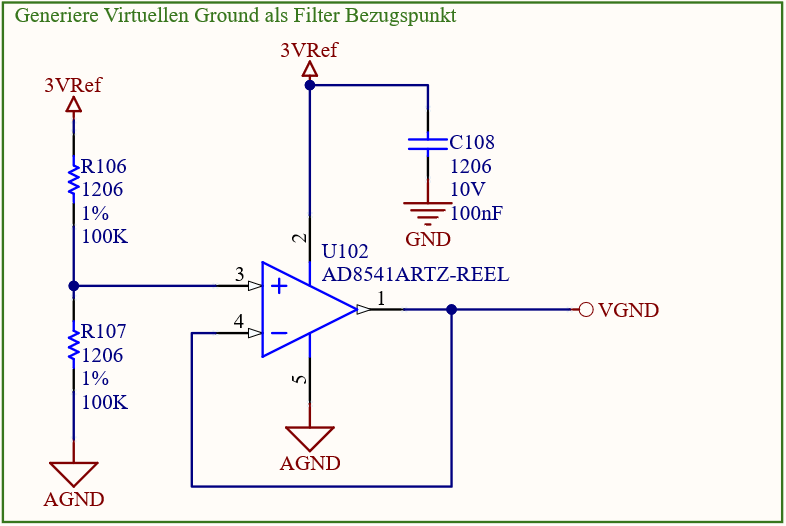
\includegraphics[width=\textwidth] {EKG_virtueller_Ground.png}
	\caption{Generierung des 1,5 V Bezugspotentials für die Filterschaltung}
	\label{Virtueller GND} 
\end{figure}

Um die Schaltung auf ein Gleichspannungspotenzial von \SI{1,5}{\volt} anzuheben wurde ein hochohmiger Spannungsteiler mit einem Operationsverstärker als Spannungsfolger verwendet (siehe Abbildung \ref{Virtueller GND}). Bei dem Operationsverstärker handelt es sich um den AD8541, den gleichen Verstärker der auch für die Filter zum Einsatz kommt.







\newpage

%ekg_7 Ergebnis

\section{Ergebnis}

Dieses Kapitel listet die Funktionen des EKG-Gerätes auf die umgesetzt werden konnten. 

\subsection{aufgenommene Signale}

Die automatisierte Aufnahmezeit der Kurzzeit-EKG Funktion wurde mithilfe einer Referenzuhr gemessen und beträgt \SI{120}{\sec}. In dieser Zeit wurden XXX Werte auf der SD-Karte, mit Zeitpunkt und Benutzerkennung gespeichert. Daraus ergibt sich eine durchschnittliche Abtastrate von XXX ($ \frac{Anzahl der Werte}{Zeit}$). Die gespeicherten ADC-Werte des EKG-Signals wurden mithilfe von MS Excel in einem Zeitdiagramm visualisiert (siehe Abbildung (Diagramm erstellen und einfügen)). Gut zu erkennen sind die P- (Vorhofkontraktion) und die T-Welle (Erregungsrückbildung der Kammern). Zwischen den beiden Wellen befindet sich der QRS-Komplex. Deutlich von einander zu unterscheiden sind die negativen (Q- und S-Zacke) und positiven Anteile (R-Zacke) des Komplexes. Aus den ADC-Werten lässt sich nun die Amplitude des Eingangssignals bei der Messung an der Hautoberfläche berechnen. Die Verstärkung der Filterschaltung wurde hierbei zur Vereinfachung als maximal (\SI{67}{\decibel}) über die gesamte Bandbreite angenommen. 
$  \frac{\frac{ADC-Breite}{delta Signalwerte} * 3V}{Verstärkung der Filterschaltung} $
Es ergibt sich eine Eingangsamplitude von XXX mV, was der EKG-Amplitude eines gesunden Menschen bei der Ableitung Einthoven 2 entspricht.

Der Test der Langzeit-Aufnahme lieferte XXX Werte. Dies entspricht einer durchschnittlichen Abtastrate von XXX.


%Kurzzeit-EKG läuft für 2 Minuten, Abtastrate etwa 250 Hz (Durchschnitt berechnen), insgesamt werden in einer Kurzzeitaufnahme etwa 30000 Werte aufgenommen, Exceldiagramm eines Signals einfügen, kein Rauschen, P- und T-Welle gut zu erkennen und zu unterscheiden, QRS-Komplex gut zu erkennen, Speicherung der rohen ADC-Werte zur späteren Auswertung auf der SD-Karte mit Timestamp und Benutzerkennung, Pulsfunktion, evtl. die Spannung des Eingangssignals zurückrechnen
%Langzeit-EKG läuft im Test 24 Stunden,  

\subsection{Akkulaufzeit, Bedienung, sonstige Funktionalität}

Stromverbrauch bei eingeschaltetem Display und voller Helligkeit etwa 220 mA
Stromverbrauch mit Display im Sleep-Modus etwa 105 - 110 mA
Stromverbrauch bei ausgeschaltetem 5V-DCDC etwa 7,7 mA
Akkustand nach einer kompletten Langzeitaufnahme war: 
Akkustand beginnt bei 100\% und sinkt danach erwartungsgemäß bis bei einer Restladung von <20\% das akustische Warnsignal ertönt

\newpage

%ekg_7 Zusammenfassung

\section{Zusammenfassung}

In diesem Kapitel werden die Zielsetzung und die tatsächlichen Ergebnisse mit einander verglichen. Außerdem werden Verbesserungen und Funktionen aufgeführt, die in einer möglichen zweiten Iteration des Projektes umgesetzt werden können.

\subsection{Was wurde erreicht}

Die grundlegende Aufgabenstellung war die Entwicklung eines Ein-Kanal-EKG-Gerätes für den mobilen Heimgebrauch. Diese Anforderung wurde erfüllt. Das EKG-Signal wird mittels Einmalelektroden an der Körperoberfläche gemessen, analog gefiltert und verstärkt und dann mit einer Frequenz von \SI{250}{\hertz} analog-digital gewandelt. Hierfür wurde das zu erwartende Signal analysiert und eine Filterschaltung entworfen. Zur Abtastung des Signals wurde ein Mikrocontroller der Firma TI programmiert. Dieser verarbeitet das Signal, die Benutzereingaben und verwaltet alle peripheren Module. 

Zur Anzeige des Signalverlaufs wurde ein Touch-Display programmiert, dass via UART vom Prozessor angesprochen wird. Das Display dient ebenso zur Steuerung und Information des Benutzers. Die Signalanzeige auf dem Display erfolgt in beiden Aufnahmemodi, kann jedoch weder in X- noch in Y-Richtung manuell skaliert werden. 

Zusätzlich zur Anzeige auf dem integrierten Display, wurde eine Android-App entwickelt. Die Kommunikation erfolgt zwischen EKG-Prozessor und Bluetoothmodul über UART und zwischen Bluetoothmodul und Smartphne über Bluetooth 2.0. In der App wird das Echtzeitsignal dargestellt und kann auch manuell skaliert werden. Weiterführende Kommunikation zwischen App und EKG-Gerät wurde nicht implementiert.

Die ADC-Werte werden vom Mikroprozessor über eine der SPI-Schnittstellen auf eine SD-Karte gespeichert. Hierfür wurde ein Kartentreiber auf dem Prozessor implementiert. Neben den Signal-Werten werden außerdem der Zeitpunkt der Messung, seit Beginn der Messung, sowie der ausgewählte Benutzer auf der jeweiligen CSV-Datei gespeichert. 

Wie geplant wurden zwei Aufnahmemodi implementiert. Im Kurzzeit-EKG wird das Signal auf dem Display und wahlweise zusätzlich in der App angezeigt. Außerdem wird die Herzfrequenz kontinuierlich berechnet und bei entsprechendem Anlass eine Warnmeldung über einen zu langsamen oder zu schnellen Puls angezeigt. Im Langzeit-EKG kann das Signal um Energie zu sparen nur auf dem integrierten Display angezeigt werden. Zudem wurde in dieser Aufnahme ein dedizierter Energiesparmodus implementiert, in dem der Prozessor die komplette Peripherie abschaltet und nur etwa alle \SI{4}{\sec} wieder anschaltet um die Daten auf die SD-Karte zu speichern. In diesem Modus ist eine Akkulaufzeit von 48 bis 60 Stunden möglich, prinzipiell sind also zwei Langzeitaufnahmen hintereinander ohne Aufladen möglich. 

Zur Energieversorgung aller Module werden über Aufwärtswandler und LDO zwei verschiedene Versorgungsspannungen aus der Akkuspannung generiert. Ebenso wurden Maßnahmen, wie Verpolschutz und Schmelzsicherungen, zum Schutz der Schaltung entwickelt. Um alle elektronischen Baugruppen zusammenzufügen wurde ein PCB mit dem Layouttool Altium erstellt und danach die Platine bei einem externen Hersteller gefertigt. Danach wurde die Platine von Hand bestückt und im Reflow-Ofen gelötet. 

Für das Gehäuse wurde mittels CAD-Programm ein Model erstellt, welches als Vorlage für den 3D-Druck diente. 

Nach den separaten Modultests, folgte die Integration aller Baugruppen und der Gesamttest. In Abbildung \ref{fig_EKG-Gerät} ist das fertige EKG-Gerät mit Elektrodenkabel abgebildet.

\begin{figure} [!h]
	%\centering
	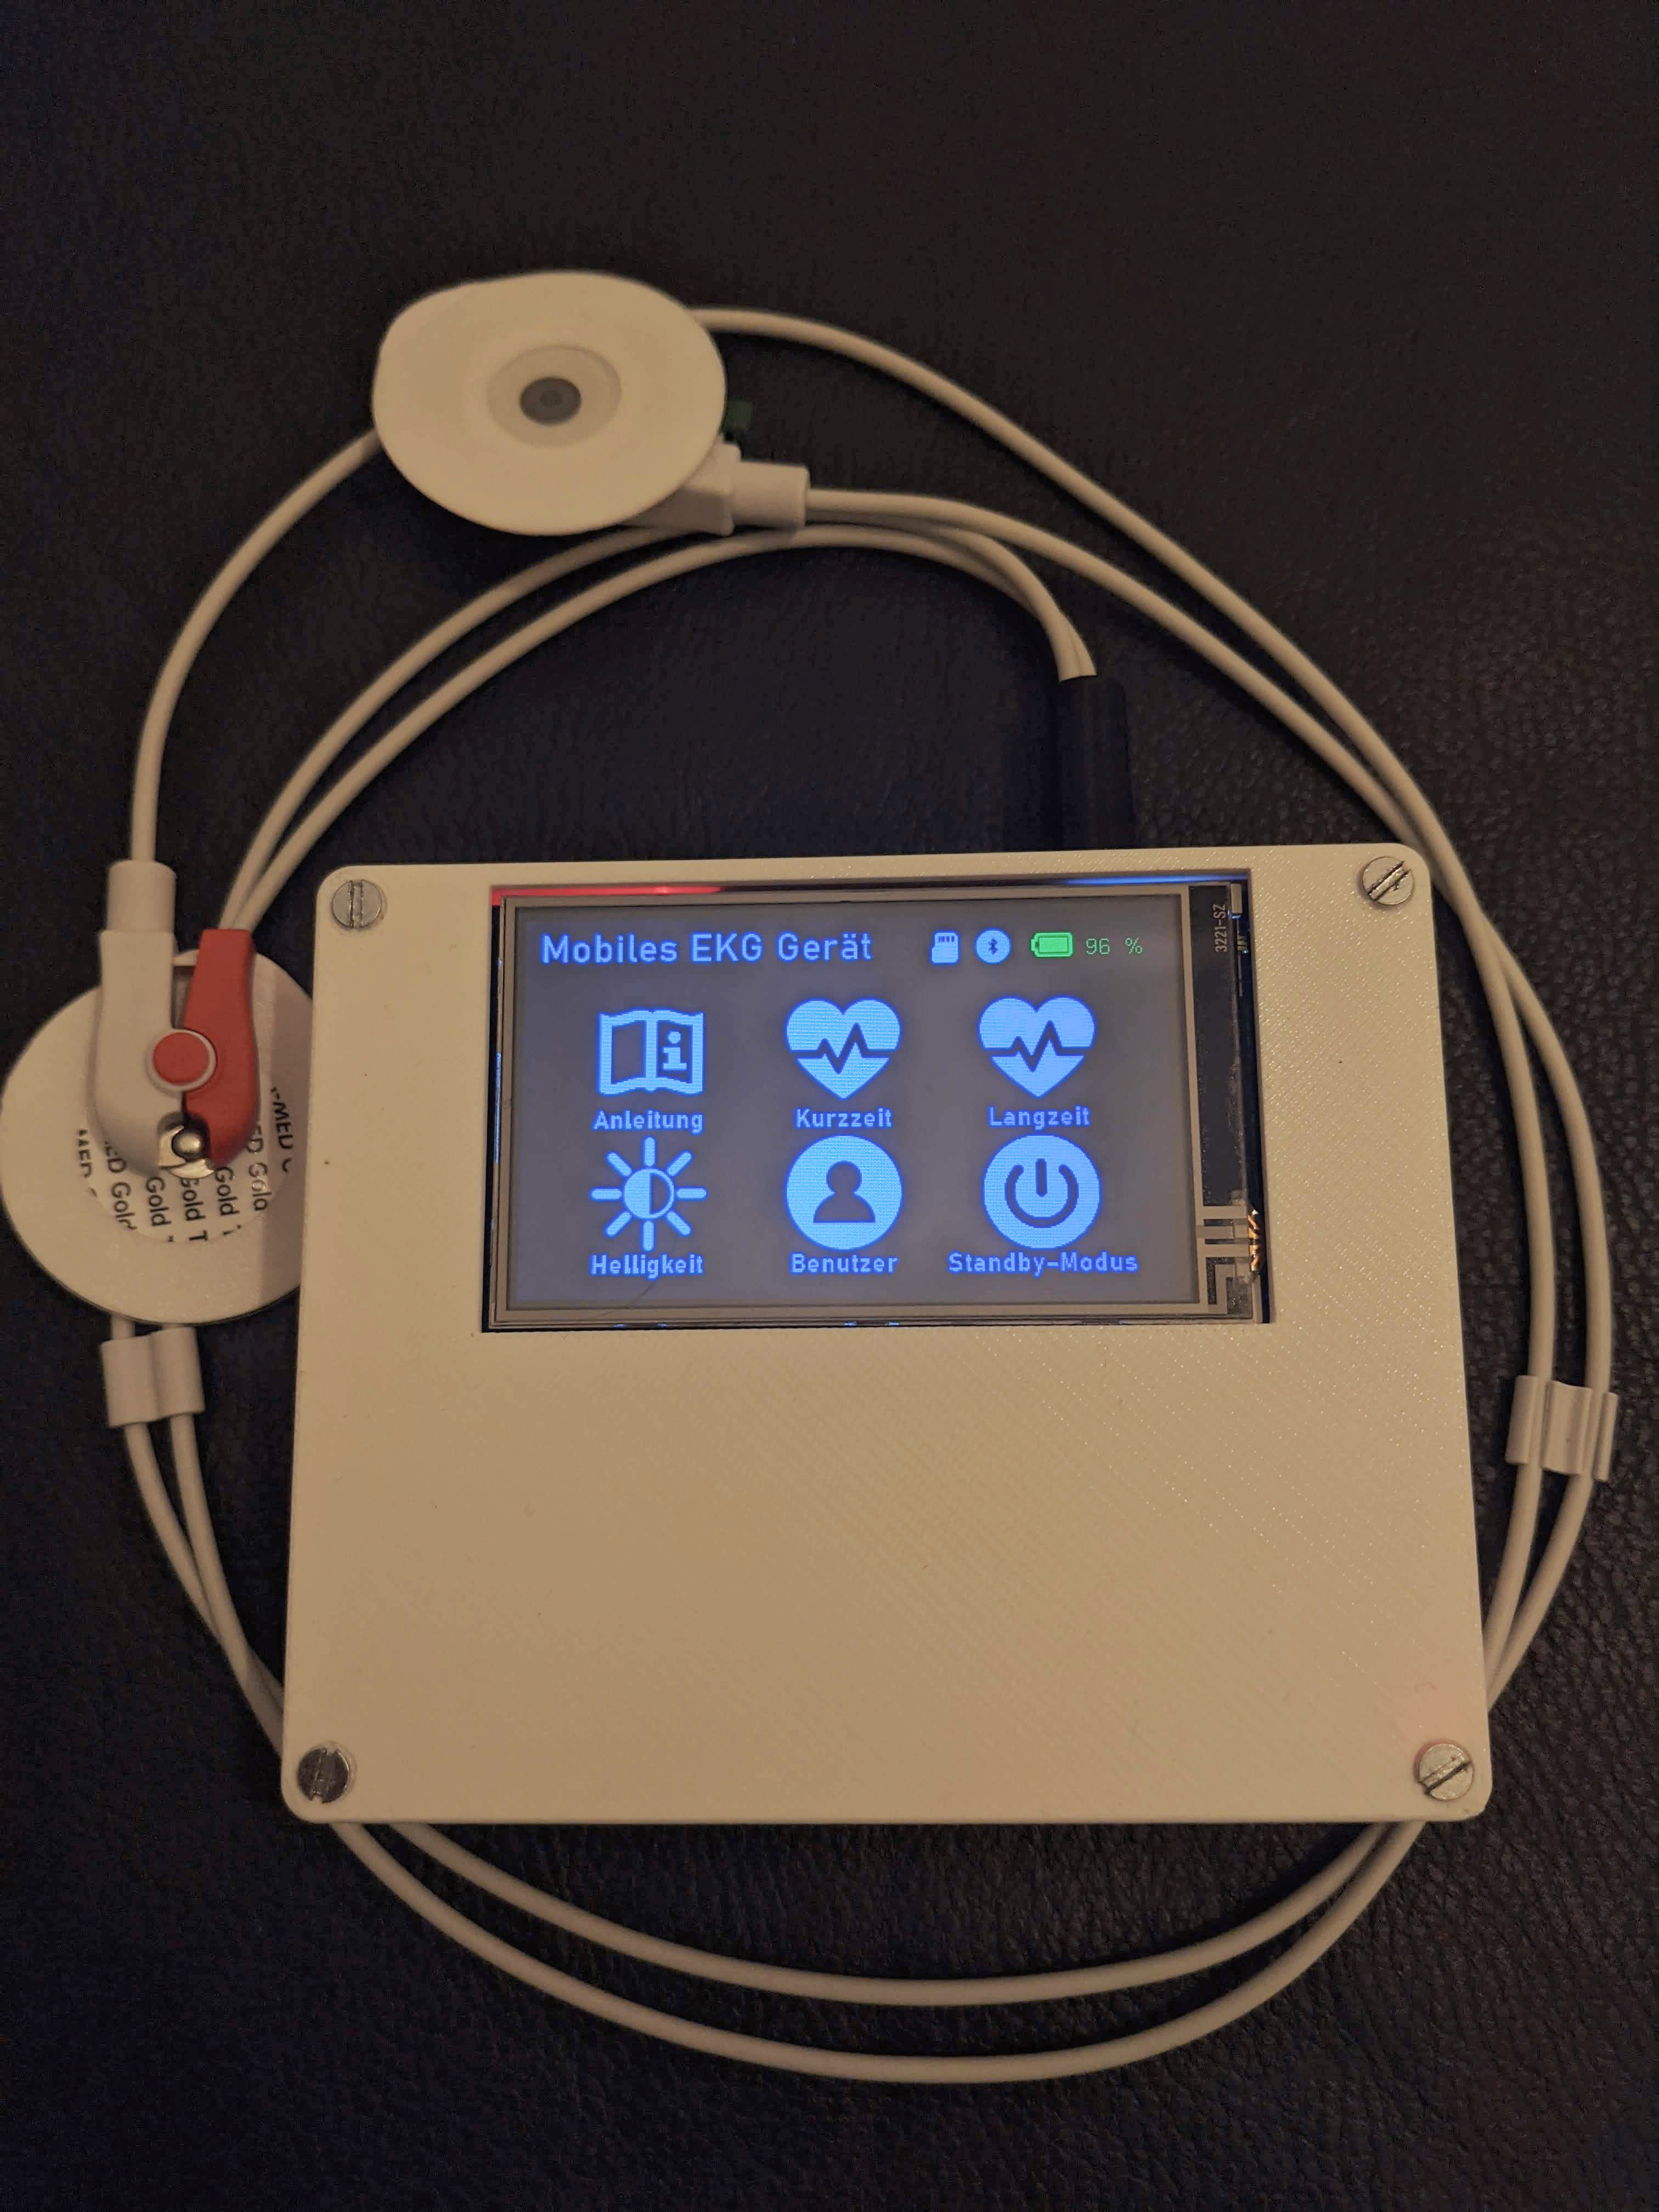
\includegraphics[width=\textwidth] {EKG_hell.jpg}
	\caption{Fertiges EKG-Gerät}
	\label{fig_EKG-Gerät} 
\end{figure}

\subsection{Ausblick/ Verbesserungen}

Während der Entwicklung wurden mögliche Verbesserungen und Erweiterungen des aktuellen Projekts aufgeworfen, die Thema dieses Unterkapitels sind.

\begin{enumerate}

\item Zur Vereinfachung der Bedienung kann die Ladeschaltung des Akkus im Gehäuse integriert werden. So kann der Benutzer auch während des Ladevorgangs das Gerät nutzen.

\item Im aktuellen Stand des Projektes liegen das Bluetooth- und SD-Karten-Modul als separate Platinen vor, die über Flachbandkabel mit der Hauptplatine verbunden werden. Die Integration dieser Baugruppen auf der Hauptplatine, würde die Störanfälligkeit der Verkabelung eliminieren und das Gehäuse könnte noch kompakter entworfen werden.

\item Um den Energiesparmodus zu vereinfachen und allgemein mehr Freiheit bei der Verwaltung der einzelnen peripheren Module zu haben, würde es sich anbieten diese separat mit Strom zu versorgen. Hierfür bieten sich Feldeffekttransistoren an, die über das GPIO-Modul des Prozessors gesteuert angesteuert werden und die Energieversorgung der Peripherie zu- oder abschalten.

\item Um die Funktionalität zu erweitern, könnte wie bereits an anderen Stelle erwähnt, ein Algorithmus zur automatisierten Diagnose von Vorhofflimmern implementiert werden. Hierfür müsste ermittelt werden ob die Rechenleistung des MSP430 bei gleichbleibender Abtastrate ausreicht, oder ob externe Leistung (z.b. Smartphone, PC) nötig ist.

\item Aktuell dient die Android-App hauptsächlich zur Anzeige des Signals. Durch eine gegenseitige Kommunikation zwischen Smartphone und EKG-Gerät könnten die Bedienmöglichkeiten des Smartphones zur Steuerung des EKG genutzt werden. Beispielsweise könnte die Tastatur eines mobilen Devices genutzt werden um die Benutzerauswahl zu erweitern und detaillierte Patientendaten auf dem EKG-Gerät zu hinterlegen.

\item Mit einem größeren integrierten Display könnten Steuerungsmöglichkeiten zur Skalierung des Signals auf dem Display implementiert werden. In der aktuellen Version wurde darauf verzichtet, da die Auswahlfelder für die eindeutige Bedienung mit dem Finger eine Mindestgröße besitzen müssen.

\end{enumerate}

\newpage
\addcontentsline{toc}{section}{Literaturverzeichnis} %fügt die Section Literaturverzeichnis zum Inhaltsverzeichnis hinzu
\bibliography{ekg_7_literatur}

%ekg_7_Anhang

\section*{Anhang}
\addcontentsline{toc}{section}{Anhang}

\end{document}